%% Springer Nature LaTeX template (sn-jnl) — Springer Basic reference style
%% Target journal: Environmental Monitoring and Assessment (Springer)
\documentclass[pdflatex,sn-basic]{sn-jnl}

%% Target journal: Environmental Monitoring and Assessment (Springer)
\usepackage{graphicx}
\usepackage{multirow}
\usepackage{amsmath,amssymb,amsfonts}
\usepackage{booktabs}
\usepackage{url}
\graphicspath{{../../results/figures/}{../}{./}}

\raggedbottom

\begin{document}

\title[Transferable satellite monitoring protocol for water transparency]{Transferable
Satellite-Based Monitoring Protocol for Water Transparency in High-Altitude
Oligotrophic Lakes: Harmonized Sentinel-2/Landsat Retrieval, Rigorous Validation and
Conformal Uncertainty in Lake Titicaca (2013--2024)}

% --- Autores ocultos de momento (para revisión del asesor). Descomentar para enviar a la revista ---
%\author[1]{\fnm{Milton Vladimir} \sur{Mamani-Calisaya}}
%\author*[1]{\fnm{Richar Andre} \sur{Vilca-Solorzano}}\email{75521963@est.unap.edu.pe}
%\author[1]{\fnm{Dina Maribel} \sur{Yana-Yucra}}
%\author[1]{\fnm{Fred} \sur{Torres-Cruz}}
%\affil*[1]{\orgdiv{Faculty of Statistical and Computer Engineering},
%\orgname{Universidad Nacional del Altiplano (UNAP)},
%\orgaddress{\city{Puno}, \postcode{21001}, \country{Peru}}}
\author{\fnm{}\sur{}}

\abstract{High-altitude Andean lakes are critical freshwater reserves that remain
poorly monitored by sparse field campaigns. We present a transferable
satellite-based protocol for monitoring water transparency (Secchi disk depth,
$Z_{SD}$) that complements in-situ programs and explicitly delimits the operational
envelope in clear oligotrophic waters. Demonstrated in Lake Titicaca (3810 m
a.s.l.) with harmonized Sentinel-2 and Landsat imagery (2013--2024) and 1002 real
satellite--field match-ups, the protocol couples a rigorous validation hierarchy,
per-pixel split-conformal uncertainty, and an explicit retrievability assessment. A
Random Forest retrieved $Z_{SD}$ with $R^2=0.64$ (RMSE 1.85 m) under station-wise
cross-validation and $R^2=0.51$ on a temporal hold-out; random and station-wise
validation were identical (no spatial-autocorrelation leakage), whereas
leave-one-zone-out extrapolation collapsed $R^2$ toward zero, and the conformal
intervals were well calibrated (89.8\% empirical coverage at a 90\% nominal level).
Chlorophyll-$a$, suspended solids and temperature were not retrievable in this
regime. The protocol produces lake-wide transparency maps that can prioritize field
sampling between campaigns and is directly transferable to other high-altitude
clear-water lakes, provided local recalibration is performed.}

\keywords{Environmental monitoring protocol, Water transparency, Secchi depth,
Sentinel-2, Landsat harmonization, Lake Titicaca, Conformal prediction,
High-altitude lakes}

\maketitle

\section{Introduction}\label{sec:intro}
Inland waters are sentinels of environmental change, yet continuous monitoring of
remote high-altitude lakes is constrained by sparse field infrastructure
\citep{Williamson2009}. Lake Titicaca, shared by Peru and Bolivia at 3810 m a.s.l.,
is a Ramsar site and the freshwater reserve for millions of Andean people, but its
water quality is documented only by infrequent field campaigns
\citep{OEFA2016,Siguayro2022eval}, even as eutrophication advances in its
near-shore bays \citep{Heredia2022,Lanza2024}.

Satellite remote sensing offers synoptic, repeatable observation
\citep{Gholizadeh2016,Topp2020}. Water transparency, quantified by the Secchi disk
depth ($Z_{SD}$) since \citet{Tyler1968}, is an integrative indicator of water
clarity strongly linked to the diffuse attenuation of light \citep{Lee2015}, and is
among the most reliably retrievable optical water-quality variables: it has been
mapped operationally from Landsat for two decades
\citep{Kloiber2002,Olmanson2008,Zhang2022}. Sentinel-2 MSI (10--60 m) and
Landsat~8/9 OLI (30 m) provide complementary revisit; their joint use requires
cross-sensor harmonization \citep{Roy2016,Claverie2018,Pahlevan2019}, and machine
learning has become the dominant tool for retrieving water-quality variables from
such harmonized constellations across many lakes
\citep{Pahlevan2020,Cao2020,Cao2022,Arias2023,Pahlevan2022,Hafeez2019,Tian2023}.
This literature, however, is dominated by turbid and productive ``Case-2'' waters,
where chlorophyll and turbidity carry a strong optical signal
\citep{Gitelson2009,Mishra2012,Nechad2010,Dogliotti2015}; clear oligotrophic
high-altitude lakes are comparatively neglected.

For Lake Titicaca specifically, prior remote-sensing work has used MODIS/Landsat
temperature and chlorophyll \citep{RuizVerdu2016}, basin-scale land-cover drivers
\citep{Baltodano2022}, automatic Sentinel-2 water products \citep{AyalaIzurieta2023},
and global remote-sensing water-quality products \citep{Maligaya2024}. None,
however, provides a harmonized multi-mission $Z_{SD}$ retrieval, local in-situ
validation at the true sampling coordinates, or an explicit assessment of which
variables are actually retrievable in its clear waters. Moreover, accuracy in this field is routinely
reported under random train/test splits that ignore spatial structure---a practice
known to inflate apparent skill when samples are spatially autocorrelated
\citep{Roberts2017,Ploton2020}---and almost never accompanied by per-prediction
uncertainty.

This study makes four contributions. First, we build, to our knowledge, the first
multi-mission harmonized $Z_{SD}$ retrieval for a high-altitude Andean lake, using
only real in-situ measurements sampled at their true coordinates. Second, we
introduce a transferable validation hierarchy (random vs. station-wise vs. temporal
vs. leave-one-zone-out) that distinguishes genuine generalization from
spatial-autocorrelation leakage and pinpoints where extrapolation fails. Third, we
attach calibrated per-pixel uncertainty via split-conformal prediction and
interpret the model with SHAP. Fourth, we transparently delimit what is not
retrievable (chlorophyll-$a$, suspended solids, temperature) in this clear-water
regime, providing a realistic operational envelope for Andean lake monitoring.

We frame this work as an environmental-monitoring tool rather than a stand-alone
retrieval exercise. The workflow developed here is a remote-sensing \emph{monitoring
protocol} designed to complement and optimize the periodic field campaigns of the
regional monitoring authorities (IMARPE, ALT and OEFA). Once calibrated against
in-situ data, it converts a sparse, costly sampling network into a near-weekly,
spatially explicit indicator of water clarity. It produces synoptic lake-wide
transparency maps with quantified per-pixel uncertainty \emph{between} field
surveys, so monitoring effort can be targeted where clarity declines or where
confidence is lowest. The protocol---match-ups, validation hierarchy, conformal
uncertainty, retrievability envelope and operational map (Fig.~\ref{fig:protocol})---is
the transferable contribution, and the Lake Titicaca retrieval is its demonstration
in a difficult clear-water, high-altitude setting.

\begin{figure}[h]
\centering
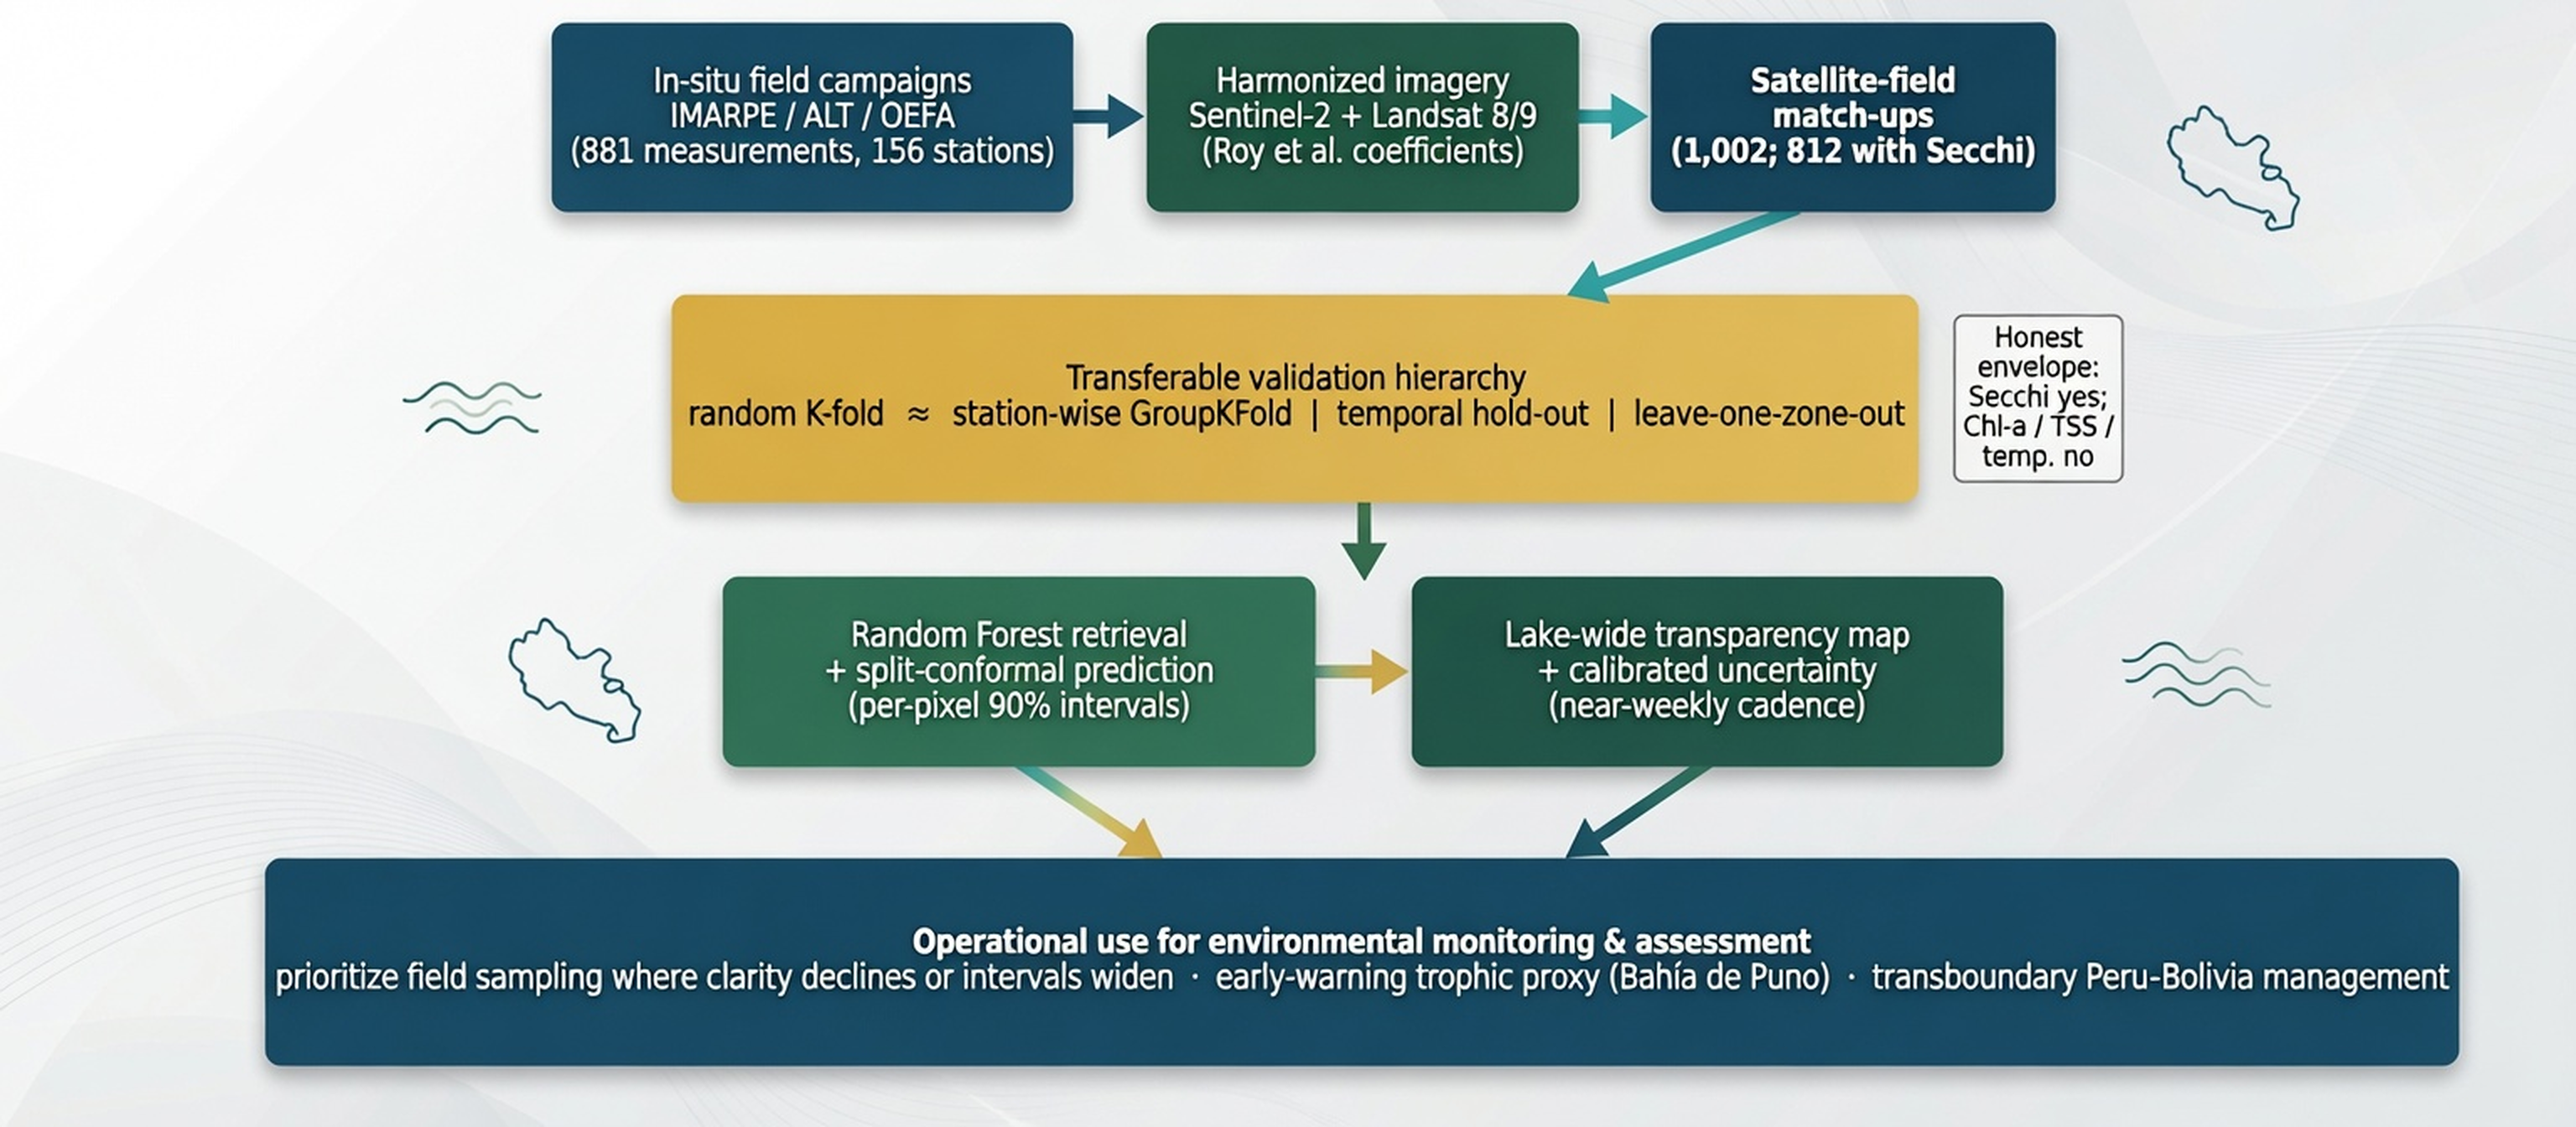
\includegraphics[width=\textwidth]{fig1_protocol.png}
\caption{Overview of the transferable monitoring protocol. In-situ campaigns and
harmonized Sentinel-2/Landsat imagery yield satellite--field match-ups; a
validation hierarchy establishes the operational envelope; a Random Forest with
split-conformal prediction produces lake-wide transparency maps with per-pixel
uncertainty; and these feed operational decisions---prioritizing field sampling,
early detection of clarity loss, and transboundary management.}\label{fig:protocol}
\end{figure}

\section{Study area and data}\label{sec:data}
\subsection{Study area}
Lake Titicaca comprises the large, deep, oligotrophic Lago Mayor; the shallower
Lago Menor (Wi\~naymarca) to the south-east; and the eutrophic Bah\'ia de Puno,
which receives municipal and agricultural inputs from the city of Puno
(Fig.~\ref{fig:study}). Transparency spans roughly 2 m in nearshore/turbid waters
to $>$15 m in the open oligotrophic basin.

\begin{figure}[h]
\centering

\includegraphics[width=0.7\textwidth]{fig_study_area.png}
\caption{Study area. In-situ monitoring stations (IMARPE/ALT), coloured by mean
measured Secchi depth, over the Natural Earth lake boundary. The spatial gradient
(clear Lago Mayor, more turbid Lago Menor and Bah\'ia de Puno) is evident in the
field data.}\label{fig:study}
\end{figure}

\subsection{In-situ data}
We used 881 real field measurements of Secchi transparency (and co-measured
chlorophyll-$a$, suspended solids, temperature, pH, dissolved oxygen and nutrients)
from the limnological monitoring campaigns of IMARPE (Instituto del Mar del Per\'u)
on Lake Titicaca, spanning 2011--2024 across 156 stations distributed over the
entire lake. Of these, 734 include a valid Secchi reading. The July~2019 campaign
(71 stations) is published by \citet{Siguayro2022data}; the remaining years derive
from the same IMARPE monitoring programme. As a provenance check, our 2019
zone-level means reproduce the published values almost exactly (e.g., Lago Mayor
conductivity 1513.4 vs. 1513.5~$\mu$S\,cm$^{-1}$; Lago Menor chlorophyll-$a$ 1.52
vs. 1.52~mg\,m$^{-3}$). Sampling is concentrated in the austral dry season
(July--October), a bias we return to in the Discussion. No synthetic or
spectrally-derived labels were used at any stage.

\subsection{Satellite data and harmonization}
Sentinel-2 MSI (harmonized surface reflectance) and Landsat~8/9 OLI (Collection~2,
Level-2 \citep{Vermote2016}) were accessed through Google Earth Engine
\citep{Gorelick2017}. Clouds were masked with the S2 Scene Classification Layer plus
cloud-probability, and with the Landsat \texttt{QA\_PIXEL} bitmask (dilated cloud,
cloud and shadow; the cirrus flag was not applied, as it is near-permanently set at
3810 m). Landsat surface reflectance was harmonized to Sentinel-2 equivalent
reflectance with the per-band linear coefficients of \citet{Roy2016}, an approach
widely used to build the harmonized Landsat/Sentinel-2 virtual constellation
\citep{Claverie2018,Pahlevan2019}. We retained the six bands common to both sensors
(B2, B3, B4, B8/NIR, B11, B12).

\section{Methods}\label{sec:methods}
\subsection{Satellite--field match-ups}
For every in-situ measurement we extracted the cloud-masked median reflectance in a
30 m buffer at the station coordinate, from imagery within $\pm$10~days
(Fig.~\ref{fig:flow}). The 30 m buffer matches the coarser Landsat pixel and
averages residual geolocation error and sensor noise over several pixels while
remaining well within open water, away from shoreline mixing; the $\pm$10-day
window balances the scarce cloud-free image availability at 3810 m against the slow
temporal change of transparency in this large, deep lake, and is consistent with
match-up windows used in operational $Z_{SD}$ retrieval \citep{Kloiber2002,Zhang2022}. This yielded 1002 real match-ups (340 Sentinel-2, 662
Landsat), of which 812 have a Secchi value across 143 stations. Because Sentinel-2
and harmonized Landsat can both observe the same field event, 272 match-ups are
cross-sensor pairs of a single in-situ measurement; collapsing them to one record
per event (540 independent events) leaves accuracy essentially unchanged
(Sec.~\ref{sec:rigor}), confirming the result is not an artefact of
pseudo-replication.

\begin{figure}[h]
\centering
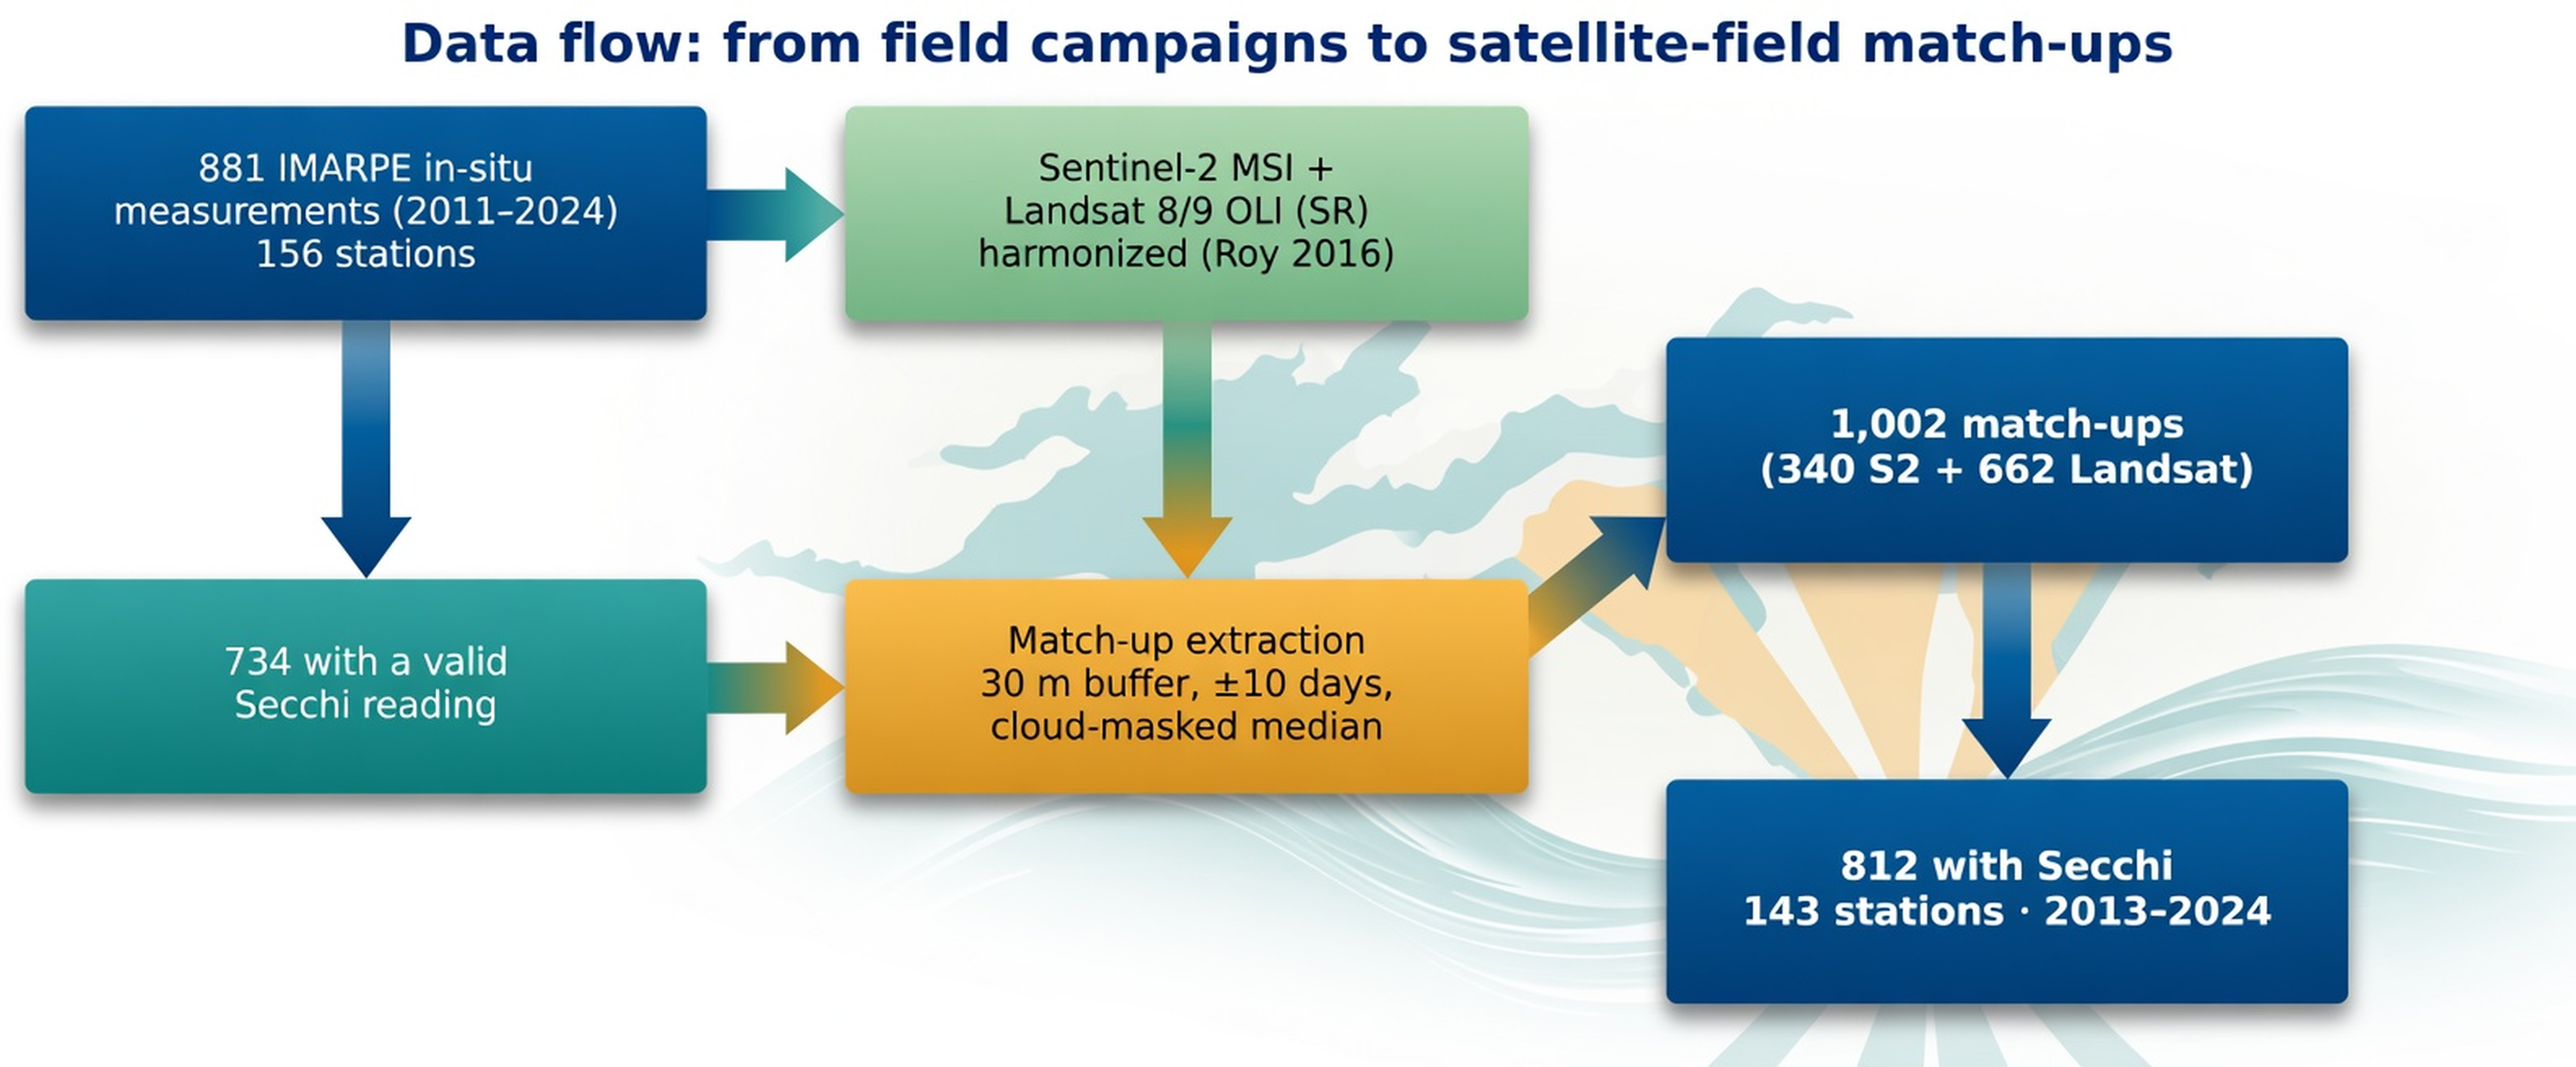
\includegraphics[width=\textwidth]{fig3_dataflow.png}
\caption{Data flow from in-situ campaigns to satellite--field match-ups. Of 881
IMARPE measurements, 734 carry a valid Secchi reading; pairing with harmonized
cloud-free imagery yields 1002 match-ups, 812 of which have a Secchi
value.}\label{fig:flow}
\end{figure}

\subsection{Features and model}
Twelve sensor-agnostic features were computed from the six harmonized bands: the
bands themselves plus NDWI, NDTI and the ratios blue/green, green/blue, red/green
and blue/red. We trained a Random Forest regressor \citep{Breiman2001} (500--600
trees, maximum depth~12, minimum 3~samples per leaf). Random Forest was preferred
over gradient boosting because it achieved the highest cross-validated accuracy
(Table~\ref{tab:perf}) while requiring minimal tuning and remaining robust at this
sample size; XGBoost \citep{Chen2016} is reported for comparison. Reflectance was
scaled with a robust (median/IQR) scaler fitted only on the training partition of
each fold, which prevents information leakage from the test data. All models were
implemented with scikit-learn \citep{Pedregosa2011}.

\subsection{Validation hierarchy}
Rather than a single split, we evaluate a hierarchy of increasingly demanding
designs \citep{Roberts2017}: (i) random K-fold; (ii) station-wise GroupKFold (5
folds), in which a station never appears in both training and test; (iii) a
temporal hold-out (train 2013--2021, test 2022--2024); and (iv) leave-one-zone-out,
in which an entire trophic zone (Bah\'ia de Puno, Lago Menor, or Lago Mayor) is
withheld, testing extrapolation to an optical regime absent from training.
Comparing (i)--(iv) separates genuine generalization from spatial-autocorrelation
leakage \citep{Ploton2020,Meyer2019}. Performance is reported as out-of-fold $R^2$,
RMSE and MAE; we benchmark against a classical log-linear blue/green band-ratio
algorithm and a multiband linear model.

\subsection{Uncertainty and interpretation}
We attach a per-prediction uncertainty interval using split-conformal prediction
\citep{Angelopoulos2023}: within each fold, a calibration subset of the training
data yields the $(1-\alpha)$ quantile of absolute residuals, which defines a
symmetric prediction interval with finite-sample coverage guarantees
\citep{Romano2019}. We report the empirical out-of-fold coverage against the nominal
level as a calibration check. The model is interpreted with SHAP
\citep{Lundberg2017,Lundberg2020}.

\section{Results}\label{sec:results}
\subsection{Retrieval performance}
The Random Forest retrieved $Z_{SD}$ with $R^2=0.64$ (Sentinel-2 only, $n=274$) and
$R^2=0.60$ (combined, $n=812$) under station-wise validation
(Table~\ref{tab:perf}, Fig.~\ref{fig:scatter}), with RMSE $\approx1.8$ m. On the
temporal hold-out (unseen years 2022--2024, including the 2023--2024 El~Ni\~no), the
model retained $R^2=0.51$ (RMSE 2.63 m), demonstrating generalization to new years.
A classical blue/green algorithm and a multiband linear model are clearly inferior
under the same station-wise design, and the Random Forest is essentially unbiased
(Table~\ref{tab:benchmark}).

\begin{table}[h]
\caption{Secchi-depth retrieval performance (station-wise GroupKFold, out-of-fold).
RMSE and MAE in metres.}\label{tab:perf}
\centering
\begin{tabular}{lcccc}
\toprule
Model / configuration & $R^2$ & RMSE & MAE & $n$ \\
\midrule
Random Forest --- Sentinel-2 only        & \textbf{0.64} & 1.85 & 1.46 & 274 \\
Random Forest --- combined (S2+Landsat)  & 0.60 & 1.81 & 1.40 & 812 \\
Random Forest --- Landsat only           & 0.58 & 1.75 & 1.33 & 538 \\
XGBoost --- combined                     & 0.57 & 1.87 & 1.44 & 812 \\
Classical blue/green ratio (log-linear, S2) & 0.39 & 2.42 & 1.91 & 274 \\
\midrule
\multicolumn{5}{l}{\textit{Temporal hold-out (train 2013--2021, test 2022--2024):}}\\
Random Forest --- combined               & 0.51 & 2.63 & 2.13 & 226 \\
\botrule
\end{tabular}
\end{table}

\begin{table}[h]
\caption{Head-to-head benchmark on the combined dataset (station-wise GroupKFold,
$n=812$). The classical band ratio fails to span the full dynamic range; the Random
Forest is accurate and nearly unbiased.}\label{tab:benchmark}
\centering
\begin{tabular}{lcccc}
\toprule
Algorithm & $R^2$ & RMSE (m) & MAE (m) & Bias (m) \\
\midrule
Classical blue/green (log-linear) & $-2.74$ & 5.51 & 1.94 & $-0.15$ \\
Multiband linear                  & 0.26 & 2.45 & 1.79 & $-0.32$ \\
Random Forest (this study)        & \textbf{0.60} & \textbf{1.81} & \textbf{1.40} & $+0.02$ \\
\botrule
\end{tabular}
\end{table}

\begin{figure}[h]
\centering
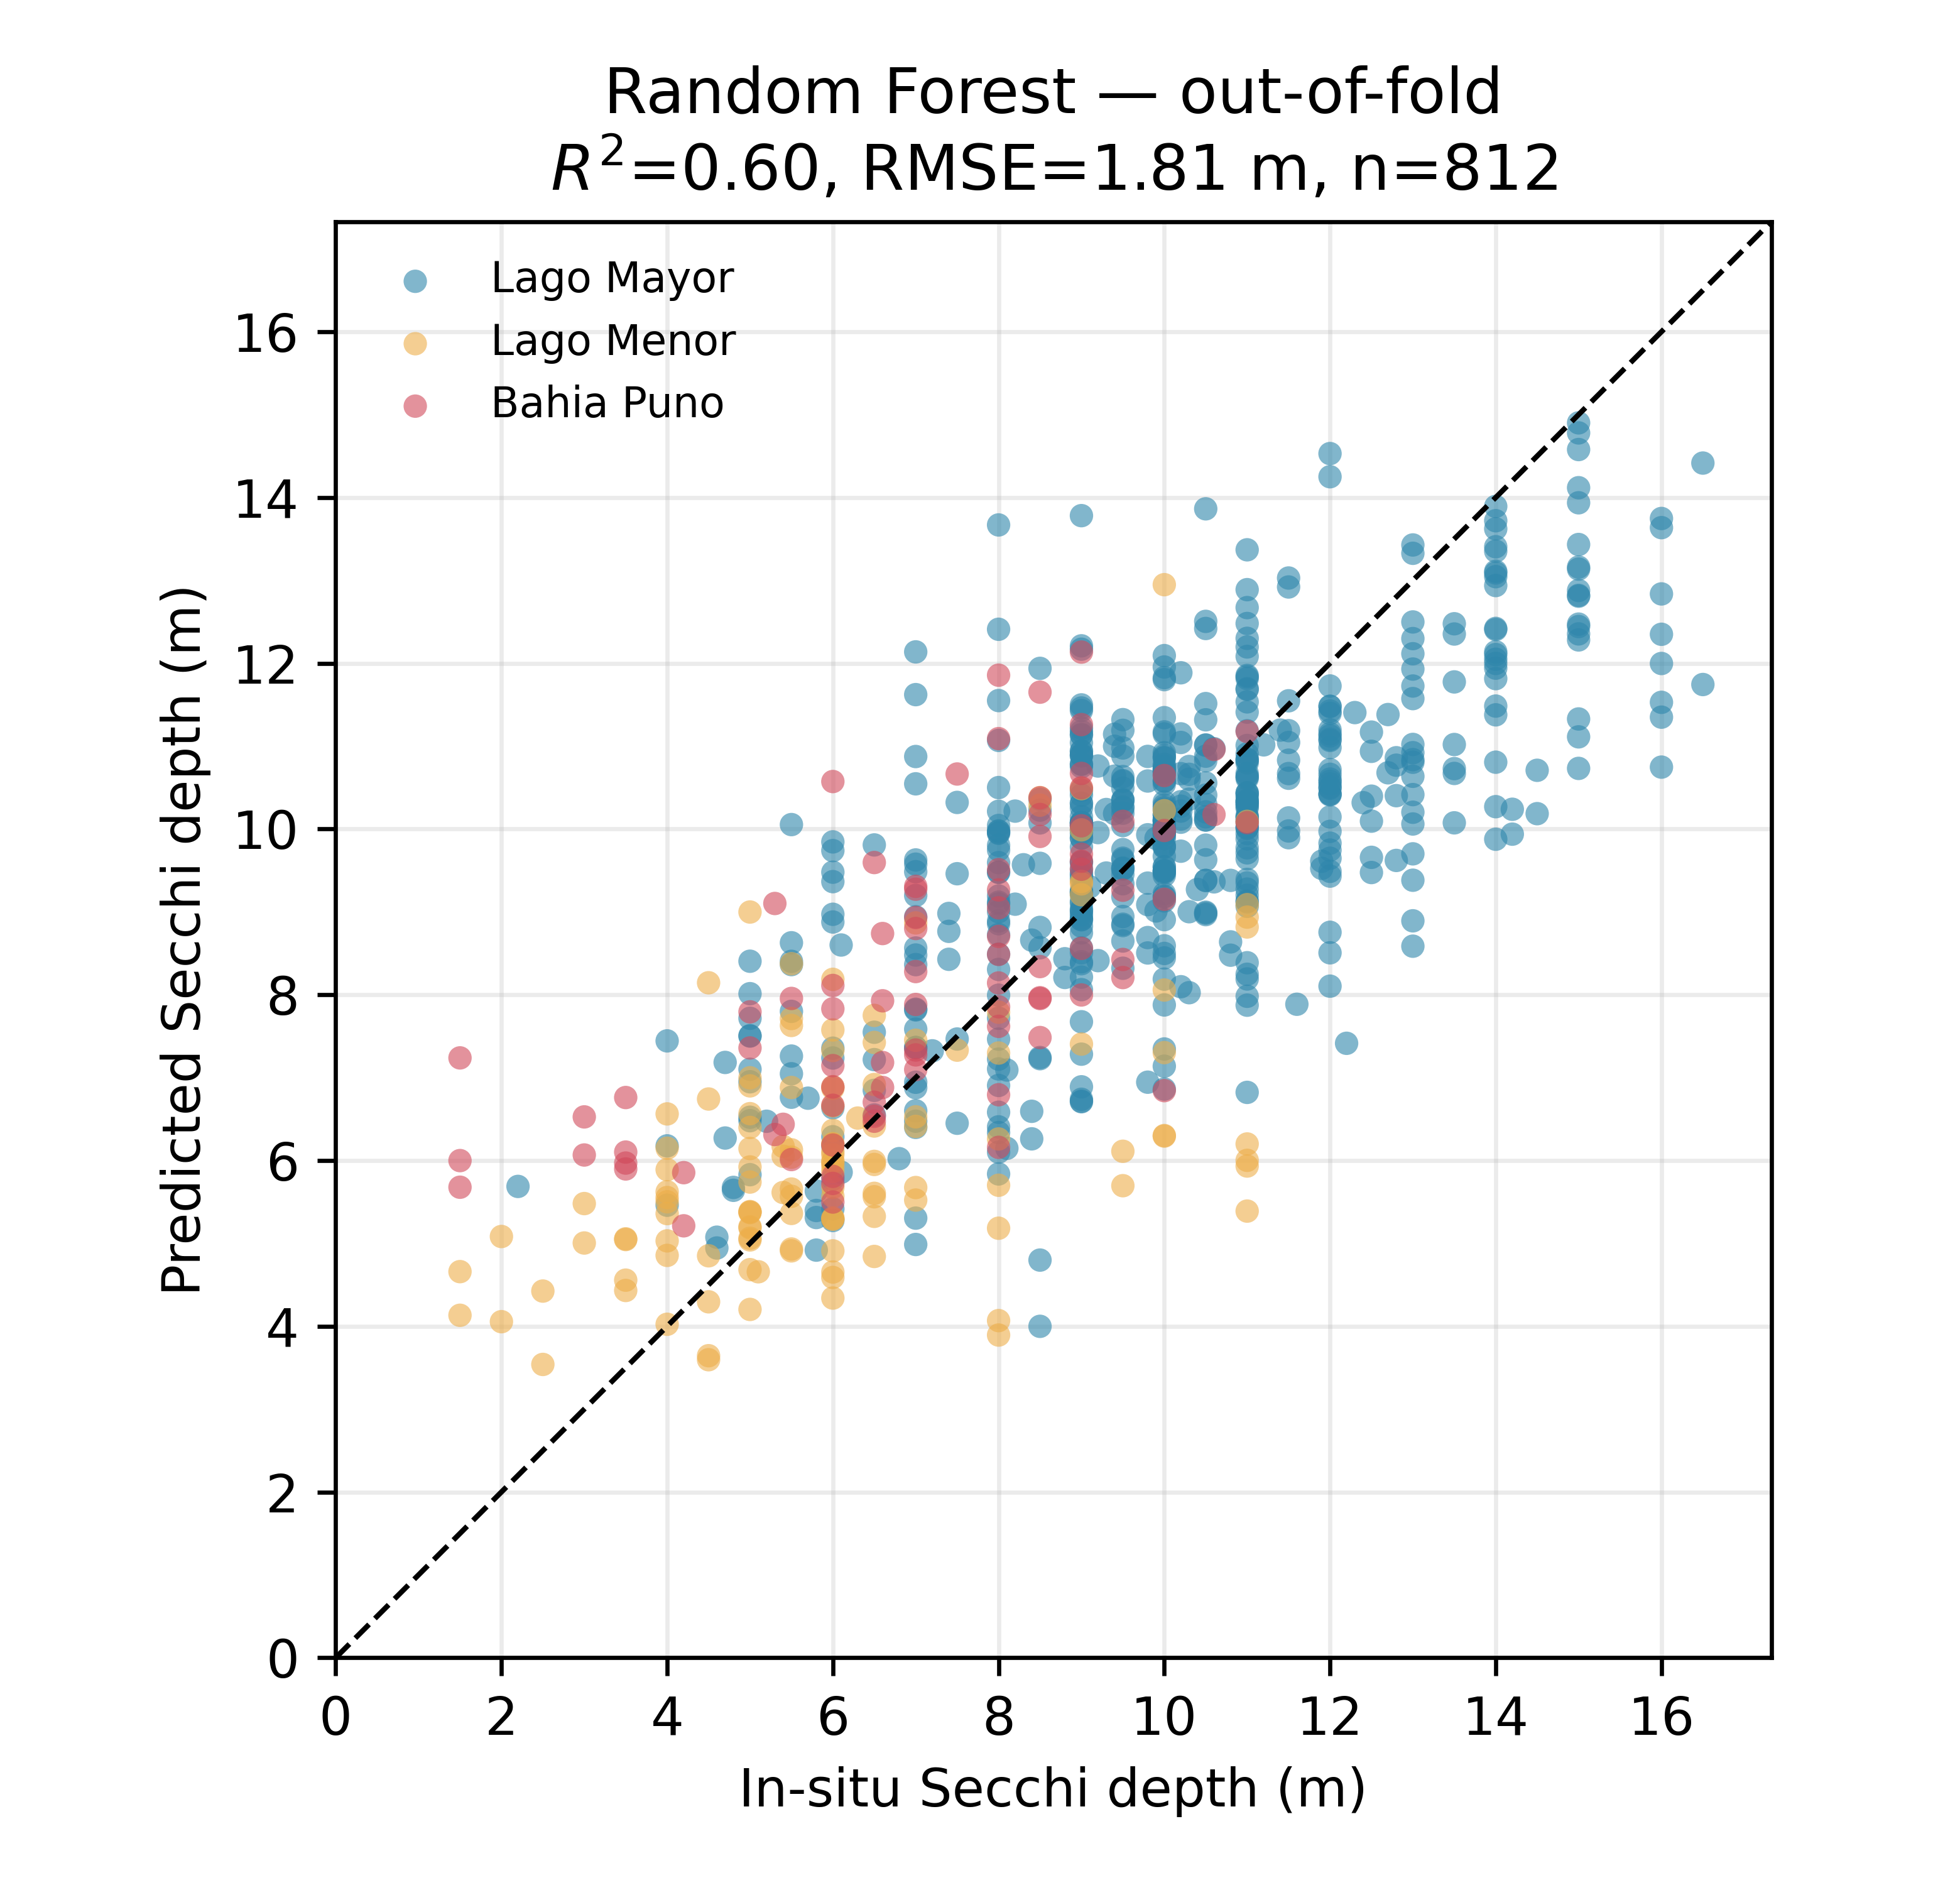
\includegraphics[width=0.7\textwidth]{fig_scatter_secchi.png}
\caption{Out-of-fold predicted vs. in-situ Secchi depth (Random Forest, combined,
station-wise validation; $R^2=0.60$, RMSE 1.81 m, $n=812$). Dashed line is 1:1;
colours denote trophic zone.}\label{fig:scatter}
\end{figure}

\subsection{A validation hierarchy: where transferability breaks}\label{sec:rigor}
Reported $Z_{SD}$ accuracy is commonly inflated by validation design and by the
sampled range. We quantify both with our own data (Fig.~\ref{fig:hier},
Table~\ref{tab:rigor}). \textit{(i) No spatial-autocorrelation leakage:} random
K-fold and station-wise GroupKFold give an identical $R^2=0.60$, so---unlike many
spatial models \citep{Ploton2020}---our retrieval does not memorize location; it
generalizes to unseen stations within the sampled regimes. \textit{(ii)
Extrapolation collapses:} withholding an entire trophic zone drops $R^2$ to 0.25
(Lago Menor), 0.04 (Bah\'ia de Puno) and $-0.05$ (Lago Mayor). The model
interpolates within optical regimes it has seen but cannot extrapolate to a water
type absent from training. \textit{(iii) Range restriction:} restricting to
homogeneous clear or turbid subsets halves $R^2$ (to $\sim0.29$) even though RMSE
improves ($\le1.5$ m). Thus a high $R^2$ can reflect a wide sampled range rather
than a better model, and RMSE is the fair cross-study metric. This hierarchy is the
transferable core of our protocol: station-wise validation is necessary but not
sufficient; only zone-out and temporal tests reveal the true operational envelope.

\begin{figure}[h]
\centering
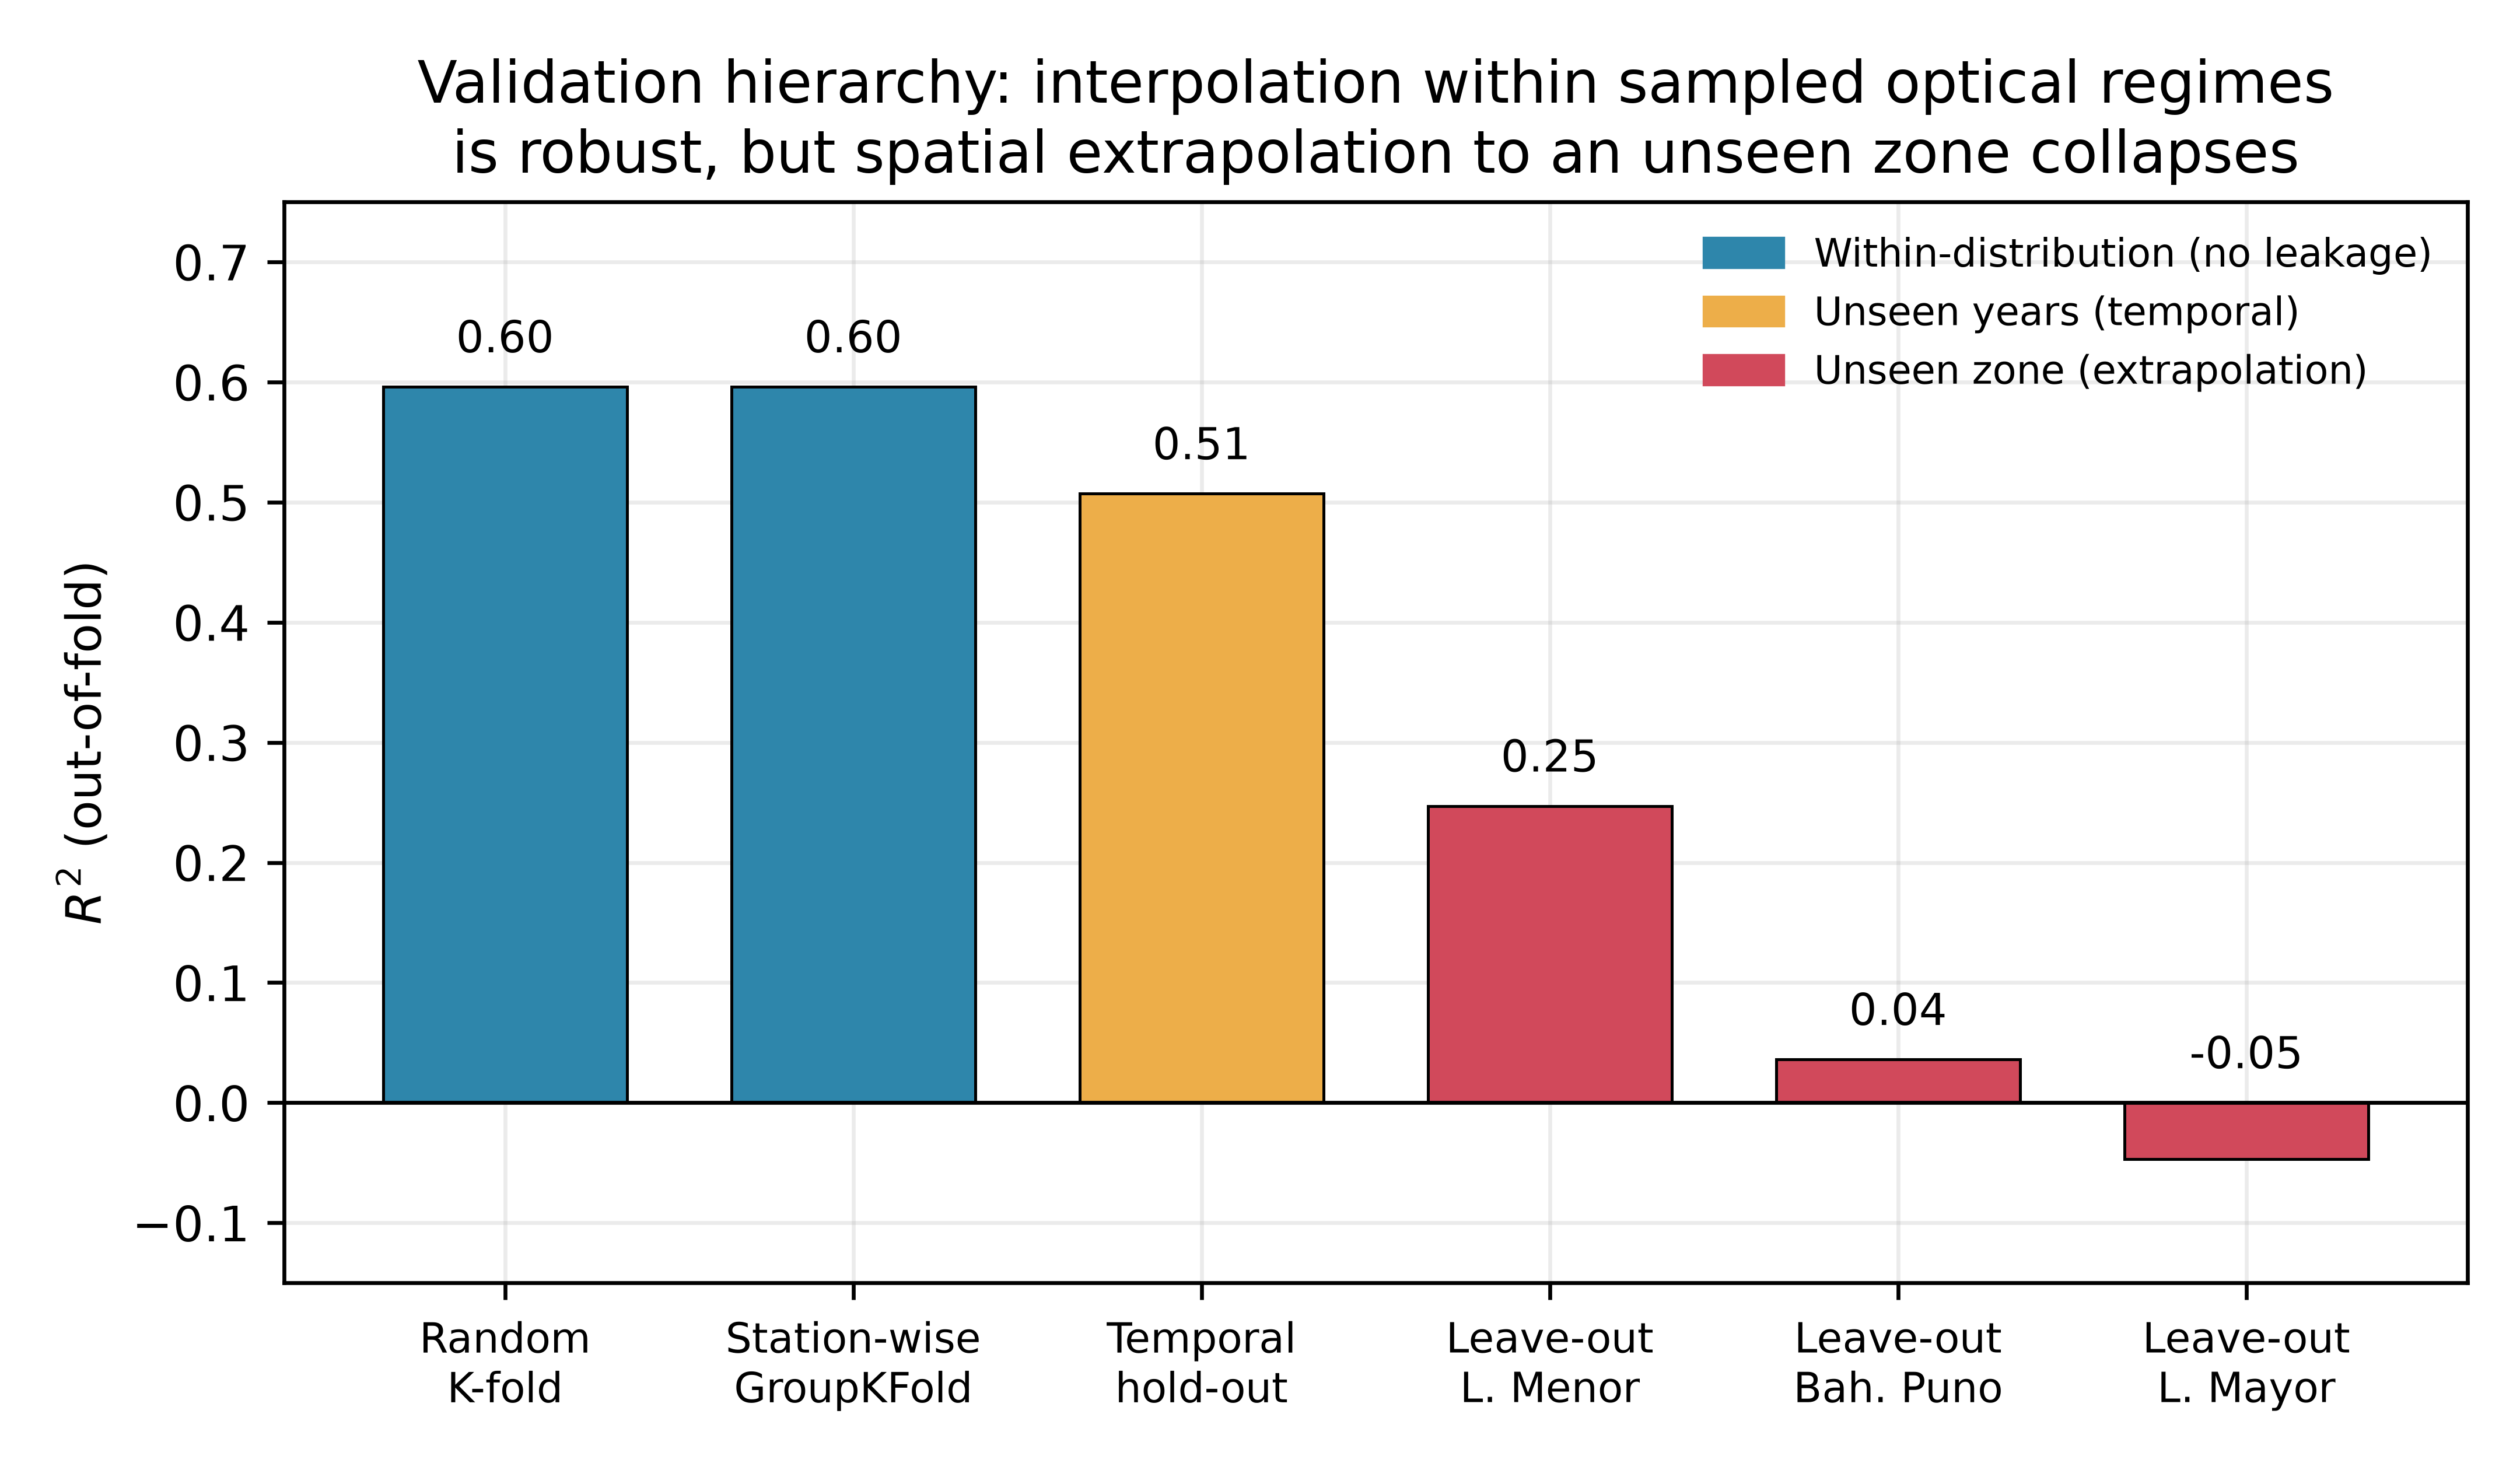
\includegraphics[width=0.85\textwidth]{fig_validation_hierarchy.png}
\caption{Validation hierarchy. Random and station-wise validation are identical (no
leakage; blue); the model generalizes across years (temporal hold-out; amber); but
extrapolation to an unseen trophic zone collapses $R^2$ toward zero (red). High
accuracy under random splits alone can therefore mask a complete loss of
transferability to new optical regimes.}\label{fig:hier}
\end{figure}

\begin{table}[h]
\caption{Validation-design and range-restriction experiments (Random Forest).
Random $\equiv$ station-wise (no leakage); zone-out extrapolation collapses; range
restriction lowers $R^2$ while RMSE improves.}\label{tab:rigor}
\centering
\begin{tabular}{lccc}
\toprule
Setting & $R^2$ & RMSE (m) & $n$ \\
\midrule
Random K-fold (leakage-prone)         & 0.60 & 1.81 & 812 \\
Station-wise GroupKFold (leakage-free)& 0.60 & 1.81 & 812 \\
One record per event (no pseudo-repl.)& 0.61 & 1.70 & 540 \\
Leave-one-zone-out: Lago Menor        & 0.25 & 1.90 & 133 \\
Leave-one-zone-out: Bah\'ia de Puno   & 0.04 & 2.11 & 88  \\
Leave-one-zone-out: Lago Mayor        & $-0.05$ & 2.52 & 591 \\
Turbid subset ($Z_{SD}<9$ m)          & 0.28 & 1.36 & 322 \\
Clear subset ($Z_{SD}\ge9$ m)         & 0.30 & 1.50 & 490 \\
\botrule
\end{tabular}
\end{table}

\subsection{Per-pixel uncertainty}
Split-conformal prediction yields well-calibrated intervals: at a 90\% nominal level
the empirical out-of-fold coverage is 89.8\%, and coverage tracks the nominal level
across the 50--95\% range (Fig.~\ref{fig:unc}). The mean 90\% interval width is
$\approx6$ m, widening in the clear basin where the optical signal saturates---a
transparent, spatially explicit statement of confidence that a single $R^2$ cannot
convey, and a prerequisite for operational use.

\begin{figure}[h]
\centering
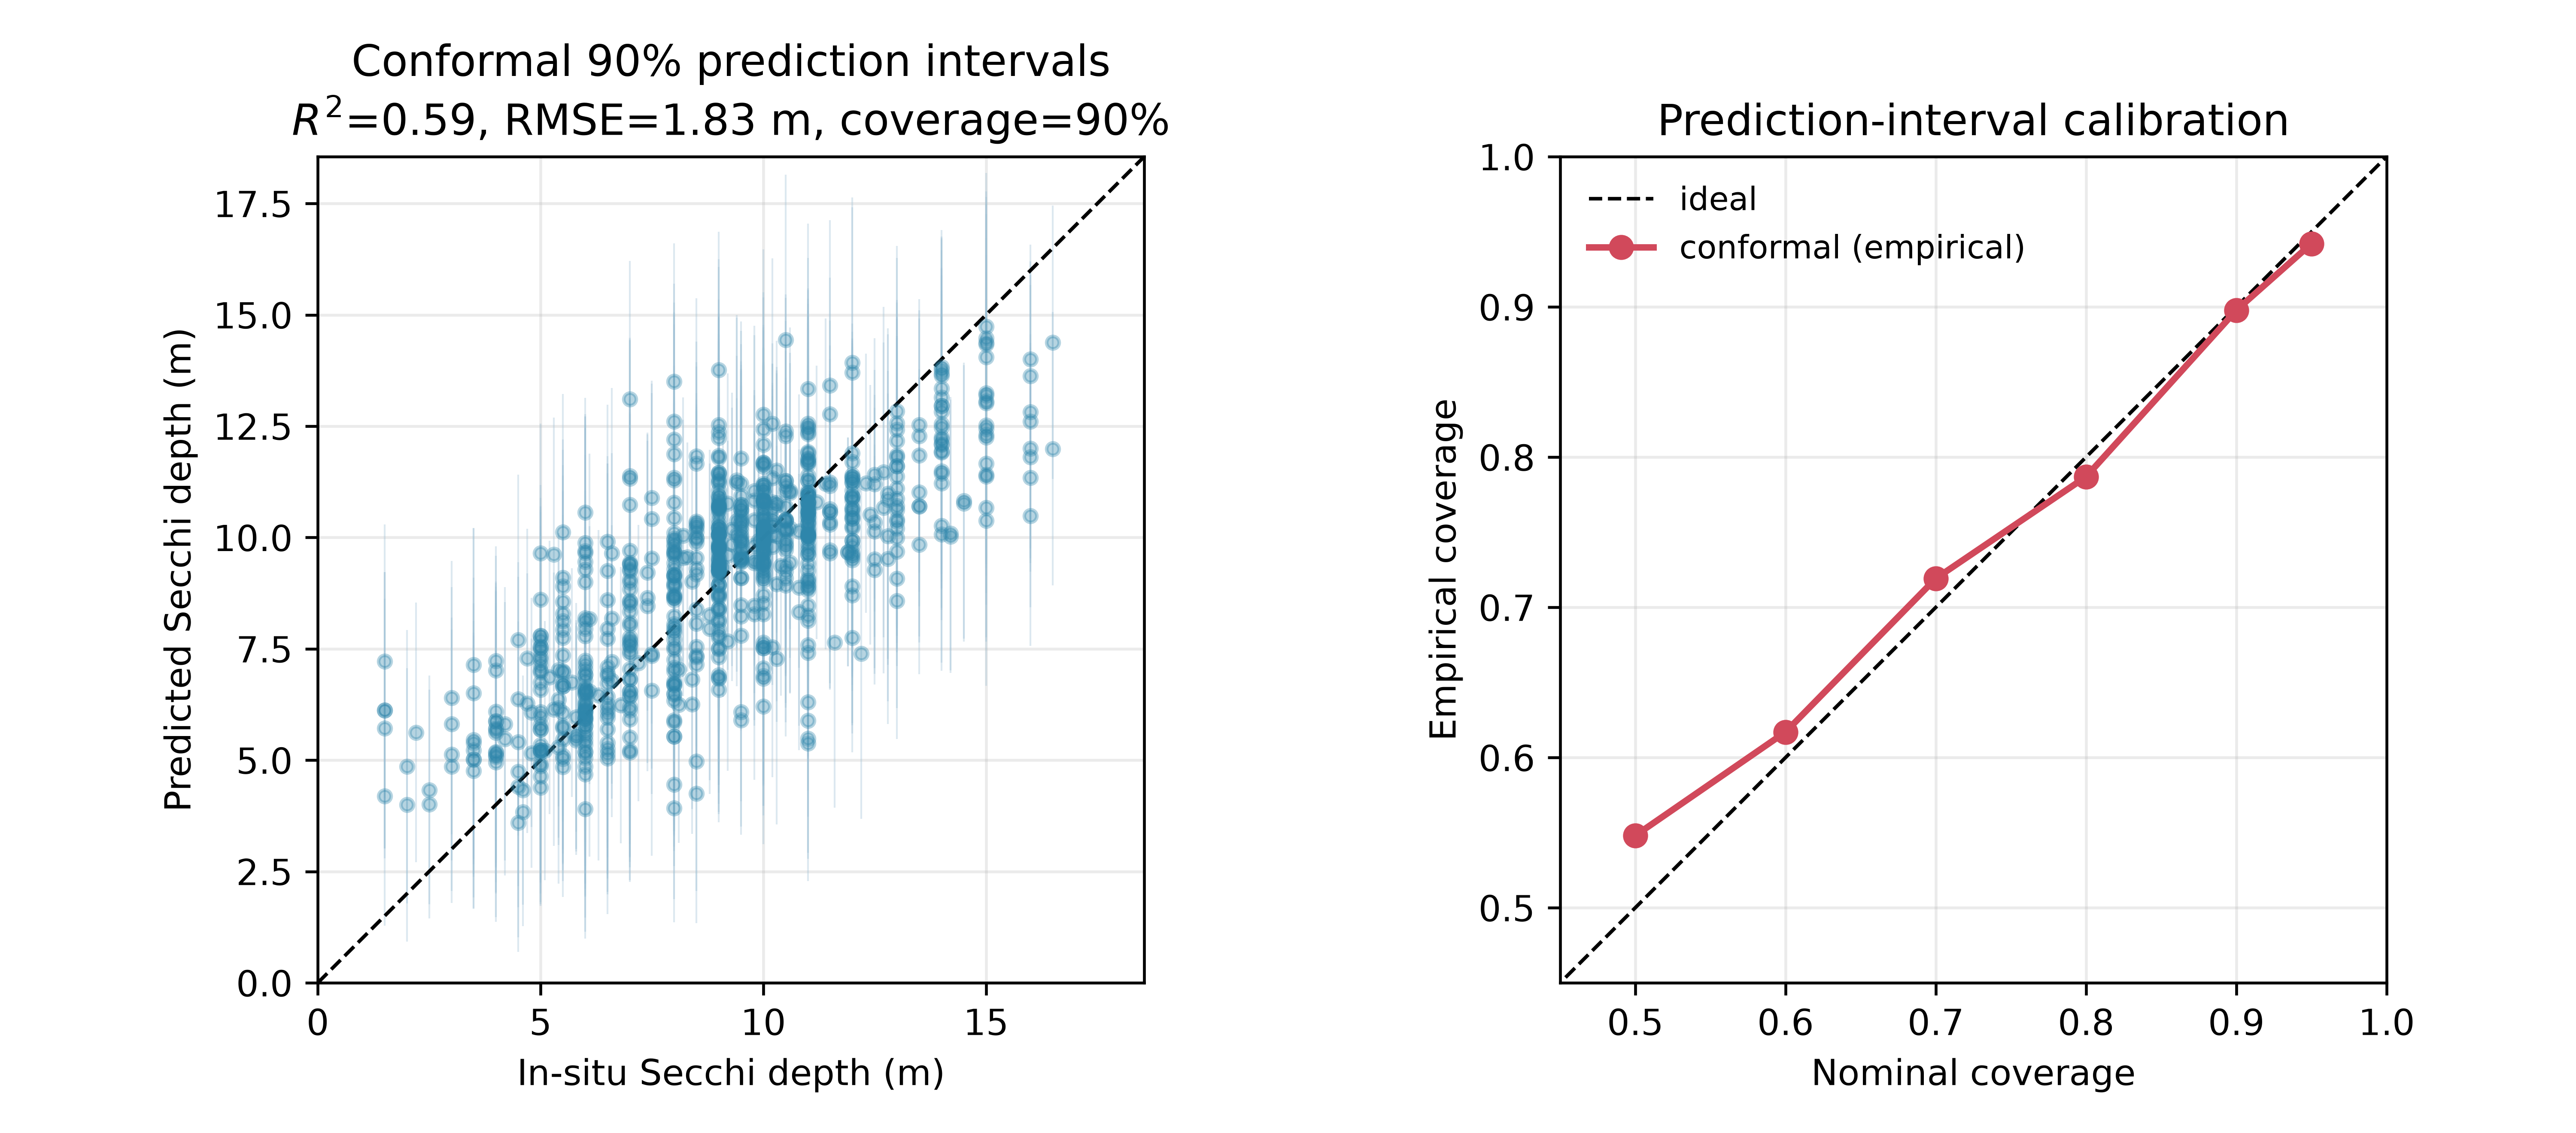
\includegraphics[width=\textwidth]{fig_uncertainty.png}
\caption{Conformal prediction intervals. Left: out-of-fold predictions with 90\%
intervals. Right: empirical vs. nominal coverage---the conformal intervals are well
calibrated (close to the 1:1 line).}\label{fig:unc}
\end{figure}

\subsection{Interpretability}
SHAP attributes the retrieval predominantly to green/blue reflectance ratios
(Fig.~\ref{fig:shap}), with secondary contributions from SWIR. This is physically
consistent: water clarity modulates the blue-to-green reflectance balance through
scattering and absorption. The retrieval is therefore grounded in optical physics
rather than location memorization, corroborating the leakage analysis of
Sec.~\ref{sec:rigor}.

\begin{figure}[h]
\centering
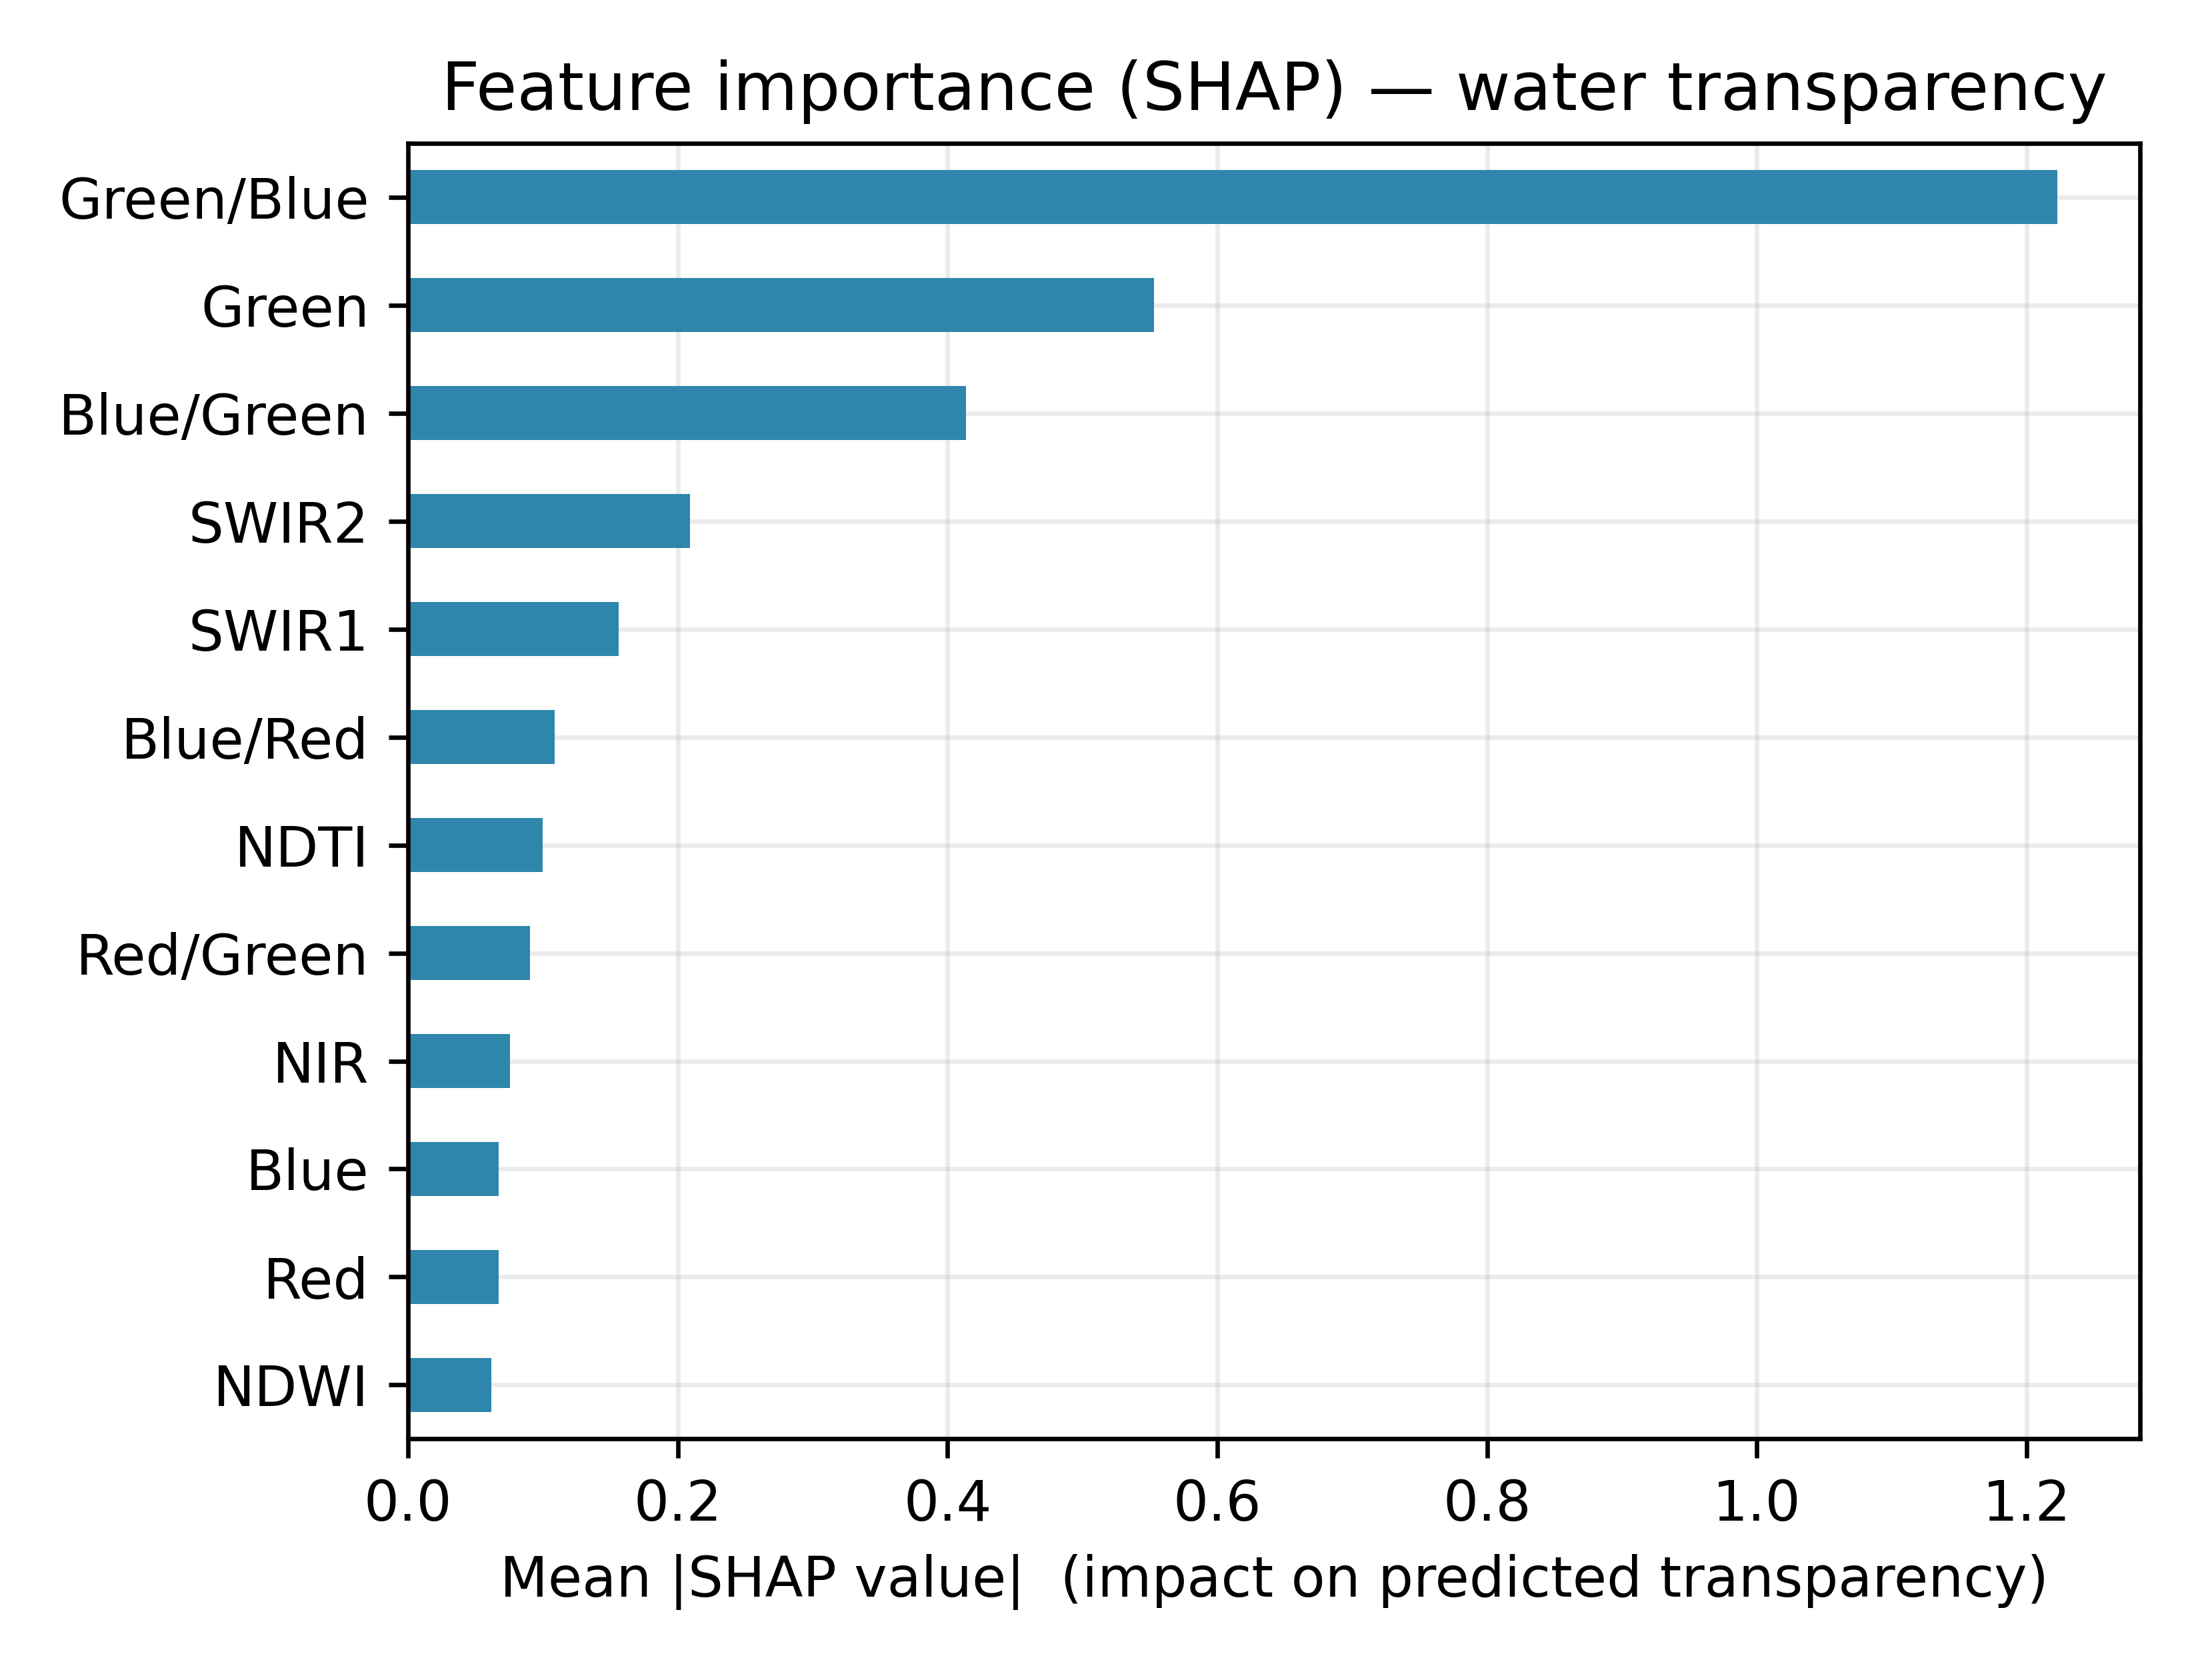
\includegraphics[width=0.7\textwidth]{fig_shap_importance.png}
\caption{SHAP feature importance for transparency retrieval. Green/blue ratios
dominate, consistent with water-clarity optics.}\label{fig:shap}
\end{figure}

\subsection{What is not retrievable}
With real labels, chlorophyll-$a$ (Pearson $r\approx0.03$ with NDCI), suspended
solids ($r=0.15$) and thermal-band surface temperature ($r=0.14$) are not
retrievable in Titicaca's oligotrophic regime: their in-situ ranges lie below the
optical/thermal detection limit. We report this explicitly to delimit the
operational envelope and to caution against applying chlorophyll algorithms
\citep{Gitelson2009,Mishra2012} or thermal retrievals \citep{RuizVerdu2016} without
local validation in clear high-altitude waters.

\subsection{Spatial and temporal patterns}
Applying the model to a 2022 dry-season Sentinel-2 composite yields a lake-wide
transparency map (Fig.~\ref{fig:map}) that reproduces the in-situ gradient: clear
Lago Mayor ($Z_{SD}\sim12$--15 m) versus more turbid Lago Menor and Bah\'ia de Puno
($\sim3$--6 m). Out-of-fold error is largest in turbid Bah\'ia de Puno (RMSE 1.95 m,
positive bias $+1.13$ m, the model pulling toward the clear-water majority) and
smallest in Lago Mayor (RMSE 1.78 m). Mann--Kendall tests on annual median in-situ
transparency (2011--2024) show no statistically significant trend in any zone
(Bah\'ia de Puno: Sen slope $+0.16$~m\,yr$^{-1}$, $p=0.24$; Lago Mayor:
$+0.25$~m\,yr$^{-1}$, $p=0.15$); continued monitoring is required
(Fig.~\ref{fig:trends}).

\begin{figure}[h]
\centering
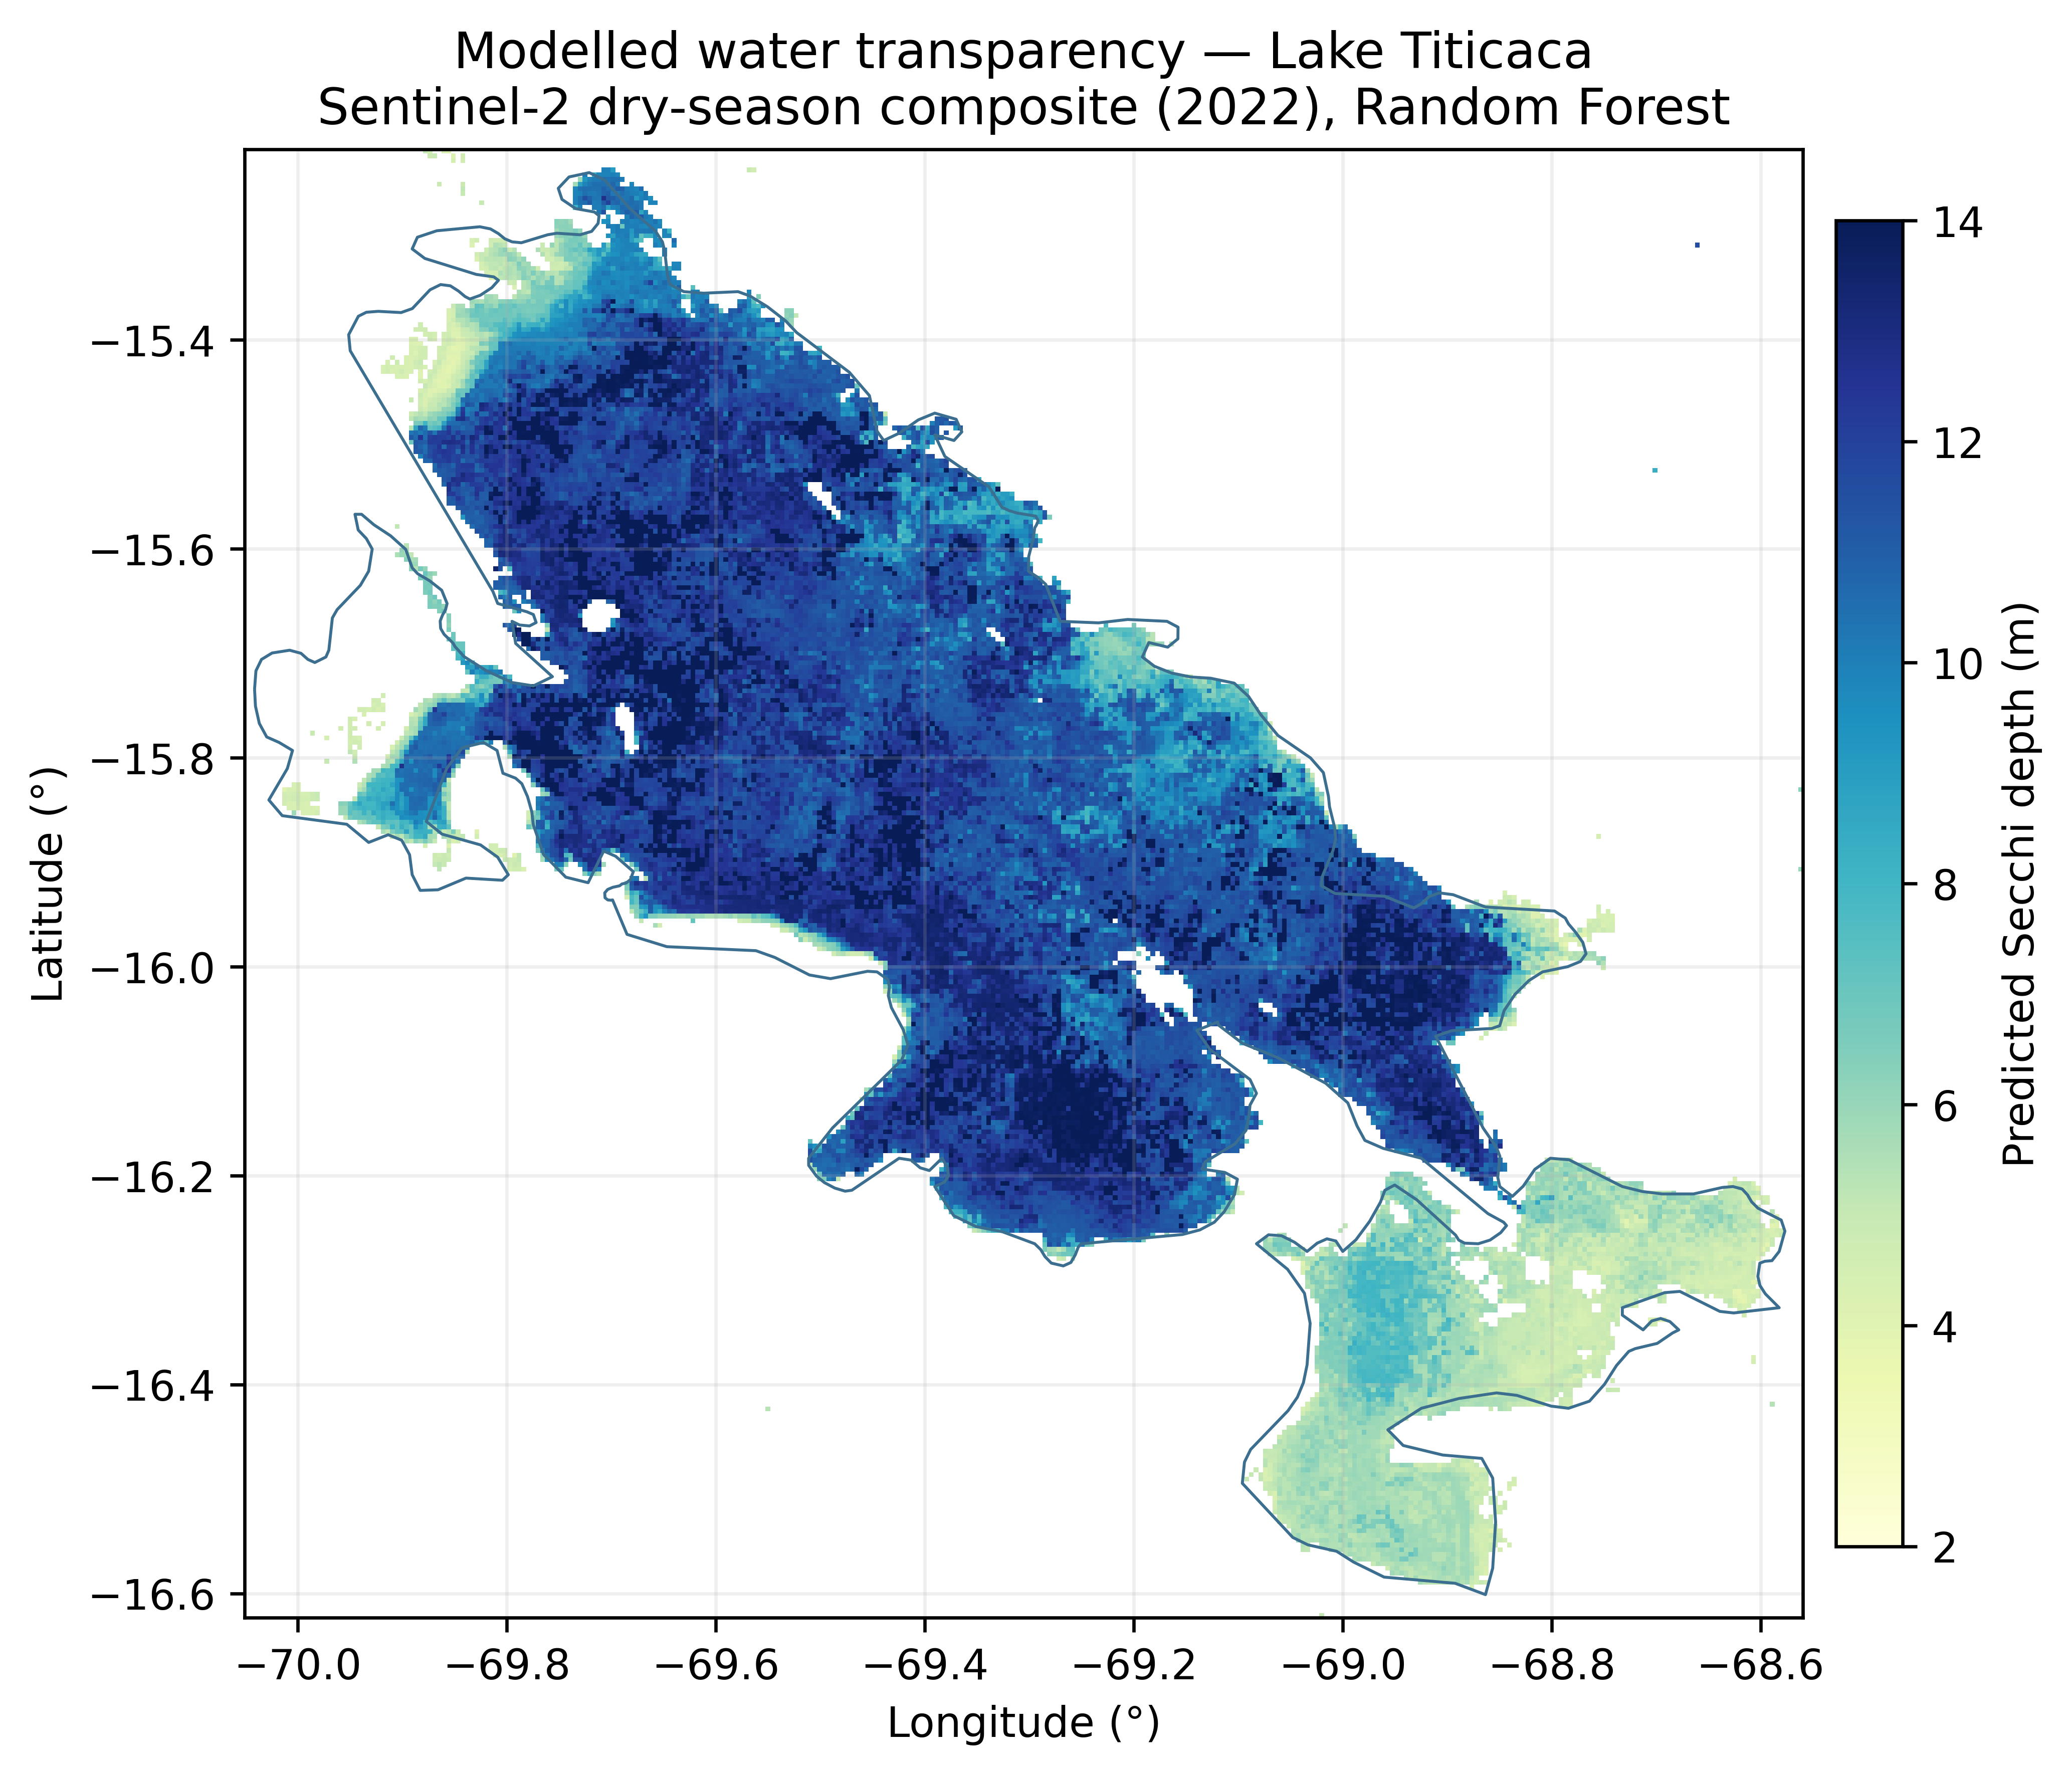
\includegraphics[width=0.7\textwidth]{fig_transparency_map.png}
\caption{Modelled water transparency (Secchi disk depth, $Z_{SD}$, in metres) from a
2022 dry-season Sentinel-2 composite; warm-to-cool colours denote turbid-to-clear
water. The spatial pattern matches the in-situ measurements (Fig.~\ref{fig:study}).
Per-pixel conformal uncertainty is quantified separately (Fig.~\ref{fig:unc}) and is
widest in the clear open basin, where the optical signal saturates.}\label{fig:map}
\end{figure}

\begin{figure}[h]
\centering
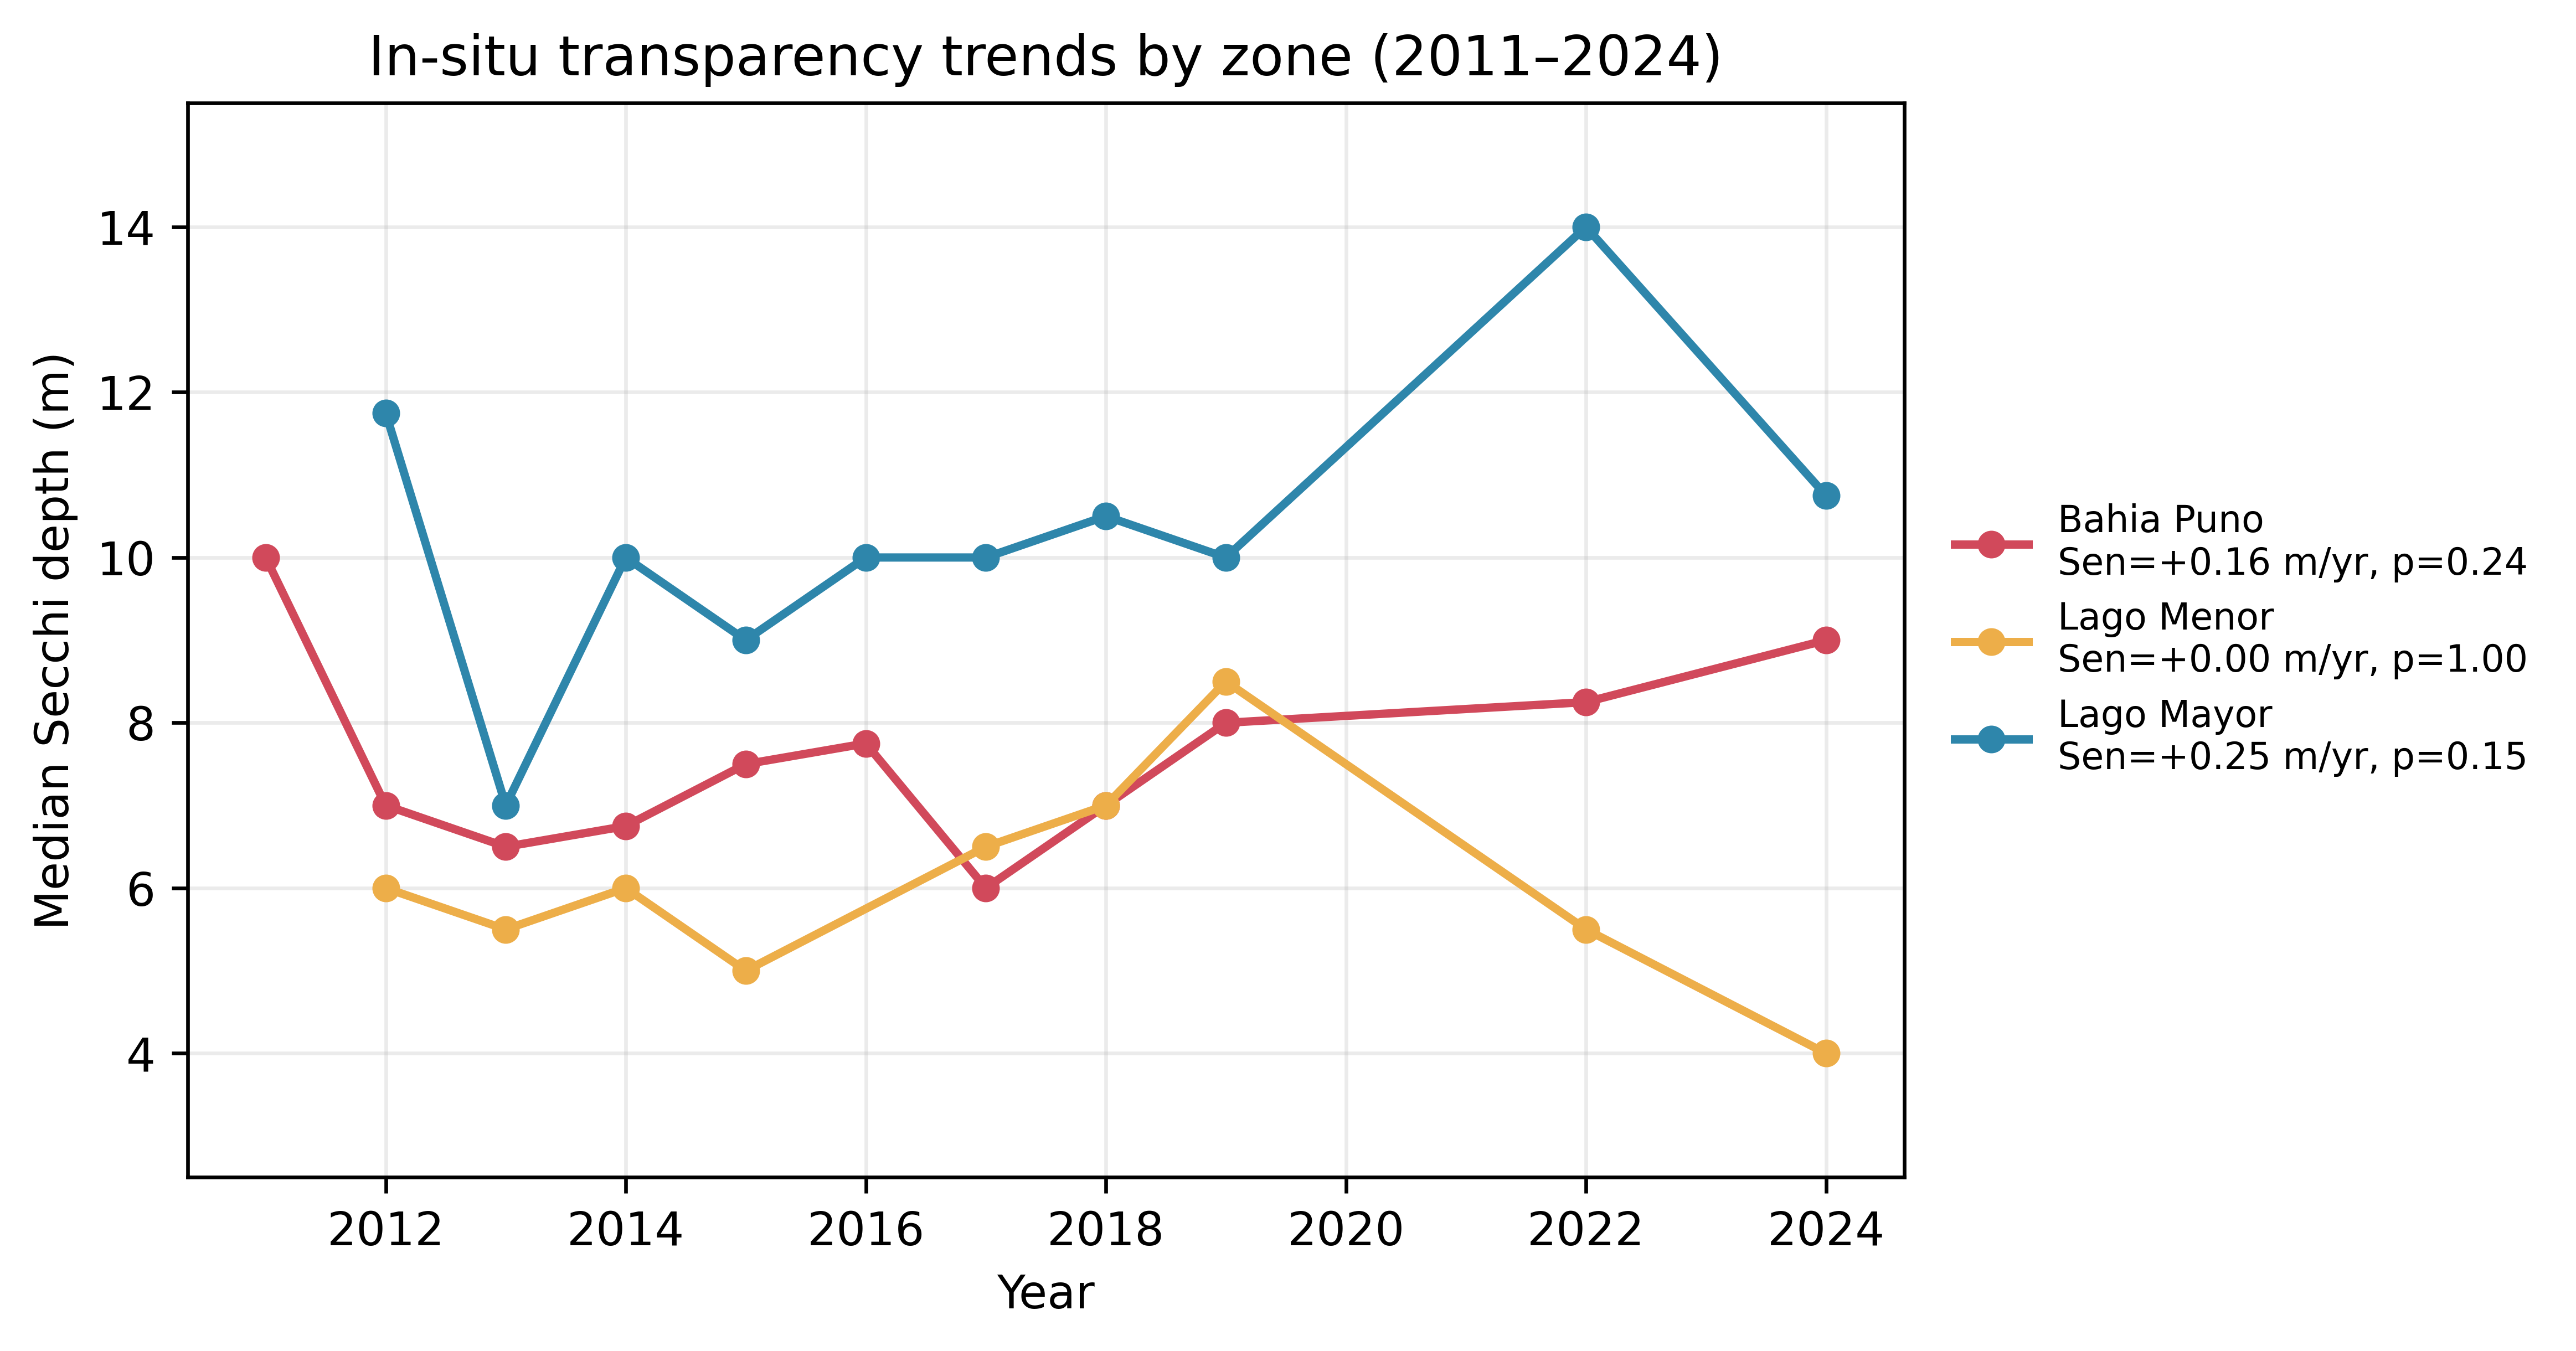
\includegraphics[width=0.75\textwidth]{fig_trends.png}
\caption{Annual median in-situ transparency by zone (2011--2024) with
Mann--Kendall/Sen statistics \citep{Mann1945,Sen1968}. No trend is statistically
significant.}\label{fig:trends}
\end{figure}

\section{Discussion}\label{sec:discussion}
Our station-wise $R^2=0.64$ (RMSE 1.8 m) sits within the published range for
$Z_{SD}$ retrieval ($R^2\approx0.6$--0.9; \citealp{Zhang2022,Lee2015}), but is
obtained under (a) a difficult, predominantly clear oligotrophic regime and (b) a
stricter, station-wise validation than the random splits common in the literature.
As our hierarchy shows, higher $R^2$ values often reflect wider sampled ranges
(turbid+clear) rather than better models, and random splits can entirely hide the
loss of skill under spatial extrapolation \citep{Roberts2017,Ploton2020}; RMSE,
reported alongside zone-out and temporal tests, is the fair comparator. The
cross-sensor signature (Fig.~\ref{fig:spectral}) confirms consistent visible bands
but a known positive bias in the harmonized Landsat NIR over dark water---an
artefact of vegetation-derived Roy coefficients \citep{Roy2016,Pahlevan2019}---which
has limited impact because the retrieval is driven by visible ratios.

\begin{figure}[h]
\centering

\includegraphics[width=0.7\textwidth]{fig_spectral_signature.png}
\caption{Mean water-leaving reflectance by sensor. Visible bands agree; the
harmonized Landsat NIR is positively biased over dark water.}\label{fig:spectral}
\end{figure}

Quantitatively, our RMSE of 1.8 m spans roughly 12\% of the observed $Z_{SD}$ range
(2--16 m), comparable to---and arguably more robust than---machine-learning $Z_{SD}$
products reported for global lakes \citep{Zhang2022} and harmonized multi-sensor
water-quality retrievals more broadly \citep{Cao2022,Arias2023,Pahlevan2022}, given
that ours is obtained under a harder clear-water regime and a stricter station-wise
validation, and is accompanied by calibrated per-pixel uncertainty that those
products generally lack.

\subsection{Operational implications for environmental monitoring}
The protocol is designed to complement, not replace, the costly periodic field
campaigns of IMARPE, ALT and OEFA. Once calibrated, it produces lake-wide
transparency maps---with per-pixel uncertainty---from freely available imagery at a
\emph{near-weekly} cadence (the combined Sentinel-2/Landsat revisit at this
latitude, before cloud loss). This is far more frequent than the typically annual or
sub-annual field surveys. In practice, persistent cloud cover---frequent during the austral
wet season (December--March)---reduces the number of usable scenes, so the realized
update frequency is lower than the nominal revisit and is itself seasonally
variable; this seasonal data availability should be reported to managers alongside
the maps. This supports three concrete monitoring functions for the regional
authorities (e.g.,\ GORE Puno, ANA, PELT and the binational ALT). First,
\emph{targeting}: the uncertainty map indicates where to send the next field
campaign---where clarity is declining or where the prediction interval is widest.
Scarce sampling effort is thereby allocated by information value rather than by
convenience. Second, \emph{early warning}: because $Z_{SD}$ integrates light
attenuation by all optically active constituents, a sustained drop in mapped
transparency is a practical first-order proxy for trophic-state change, most
relevant in the eutrophying Bah\'ia de Puno. Third, \emph{transboundary
consistency}: a single harmonized product covers the whole Peru--Bolivia lake under
one calibration, supporting comparable assessment across the international boundary
where coordinated field monitoring is logistically hard.

Two caveats bound this operational use. The retrieval carries a positive bias in
turbid Bah\'ia de Puno ($+1.13$~m; Sec.~\ref{sec:results}), because the
clear-water majority pulls predictions upward---precisely the most vulnerable zone,
so mapped values there should be read together with their (wider) uncertainty
interval and confirmed by field sampling rather than taken at face value. And, as
the leave-one-zone-out experiment shows, the model interpolates within sampled
optical regimes but does not extrapolate to an unseen water type. Integration is
therefore intended to be incremental---each new campaign both validates the current
map and extends the training set, progressively widening the operational envelope.
This is the single most important condition for safe operational use:
\textbf{the protocol must not be transferred to a new lake, or to an unsampled
optical sub-basin, without a prior local recalibration against field
data}---applying it blindly would risk confidently wrong maps in precisely the
conditions where managers most need reliable information.

The explicit delimitation of non-retrievable variables is itself a result: it warns
that chlorophyll/turbidity products transferred from turbid lakes can be physically
meaningless in clear high-altitude waters. Three further limitations bound the
results: the field data are dry-season biased, so wet-season blooms in Bah\'ia de
Puno are under-represented and future work should add rainy-season campaigns;
transparency above $\sim$15 m saturates the signal; and the harmonized Landsat NIR
bias should be locally recalibrated against simultaneous Sentinel-2 overpasses.

\section{Conclusions}\label{sec:conclusions}
A harmonized Sentinel-2/Landsat Random Forest retrieves water transparency in
high-altitude Lake Titicaca with well-validated accuracy ($R^2=0.64$, RMSE 1.8 m) under
strict station-wise and temporal validation, driven by physically meaningful
green/blue optics, and accompanied by calibrated per-pixel uncertainty. Beyond the
retrieval itself, our central contribution is a transferable protocol: a validation
hierarchy (random $\to$ station $\to$ temporal $\to$ zone-out) that distinguishes
generalization from leakage and reveals where extrapolation fails; conformal
prediction intervals; and an explicit retrievability assessment that delimits which
variables can and cannot be recovered in clear oligotrophic water. We provide a
reproducible, openly archived pipeline and a lake-wide transparency map. By
delivering maps with calibrated confidence \emph{between} field campaigns, the
protocol turns intermittent in-situ sampling into a continuous, decision-ready
monitoring indicator for the management of these vulnerable Andean freshwater
reserves. It is directly transferable to other high-altitude oligotrophic lakes
worldwide, where clear-water optics challenge water-quality algorithms calibrated on
turbid systems. In practical terms, it gives Andean lake managers a low-cost,
continuously updated instrument to detect clarity loss early and act before
degradation becomes irreversible---a concrete contribution to the environmental
monitoring and assessment of these transboundary high-altitude freshwater reserves.

\backmatter

\bmhead{Acknowledgements}
We thank IMARPE, ALT and OEFA for the publicly available monitoring records that
made this study possible.

\section*{Declarations}

\noindent\textbf{Funding} This research received no external funding.

\noindent\textbf{Competing interests} The authors declare that they have no
competing interests.

\noindent\textbf{Ethics approval and consent to participate} Not applicable.

\noindent\textbf{Consent for publication} Not applicable.

\noindent\textbf{Data availability} The real satellite--field match-up datasets
analysed in this study are openly available in the repository
\url{https://github.com/Andre031222/harmonized-titicaca-transparency}. Raw imagery
is freely available via Google Earth Engine; the in-situ measurements derive from
published IMARPE/ALT and OEFA monitoring records.

\noindent\textbf{Code availability} All processing and modelling code is openly
available at \url{https://github.com/Andre031222/harmonized-titicaca-transparency}.

\noindent\textbf{Author contributions} R.A.~Vilca-Solorzano led the data
processing, modelling and analysis and wrote the manuscript; M.V.~Mamani-Calisaya
and D.M.~Yana-Yucra contributed to data curation and validation; F.~Torres-Cruz
supervised the work and reviewed the manuscript. All authors read and approved the
final manuscript.

\bibliography{references}

\end{document}
